\documentclass[]{article}
\usepackage{amssymb,amsmath}
\usepackage{ifxetex,ifluatex}
\usepackage[english]{babel}
\ifxetex
  \usepackage{fontspec,xltxtra,xunicode}
  \defaultfontfeatures{Mapping=tex-text,Scale=MatchLowercase}
\else
  \ifluatex
    \usepackage{fontspec}
    \defaultfontfeatures{Mapping=tex-text,Scale=MatchLowercase}
  \else
    \usepackage[utf8]{inputenc}
  \fi
\fi
\usepackage{graphicx}
% We will generate all images so they have a width \maxwidth. This means
% that they will get their normal width if they fit onto the page, but
% are scaled down if they would overflow the margins.
\makeatletter
\def\maxwidth{\ifdim\Gin@nat@width>\linewidth\linewidth
\else\Gin@nat@width\fi}
\makeatother
\let\Oldincludegraphics\includegraphics
\renewcommand{\includegraphics}[1]{\Oldincludegraphics[width=\maxwidth]{#1}}
\ifxetex
  \usepackage[setpagesize=false, % page size defined by xetex
              unicode=false, % unicode breaks when used with xetex
              xetex,
              colorlinks=true,
              linkcolor=black]{hyperref}
\else
  \usepackage[unicode=true,
              colorlinks=true,
              linkcolor=black]{hyperref}
\fi
\hypersetup{breaklinks=true, pdfborder={0 0 0}}
\setlength{\parindent}{0pt}
\setlength{\parskip}{6pt plus 2pt minus 1pt}
\setlength{\emergencystretch}{3em}  % prevent overfull lines
\setcounter{secnumdepth}{0}

\begin{document}

\begin{titlepage}
\centering \parindent=0pt
\newcommand{\HRule}{\rule{\textwidth}{1mm}}
\vspace*{\stretch{1}} \HRule\\[1cm]\Huge\bfseries
Simple Gaze Tracker\\[0.7cm]
\large SIGB Assignment 1\\[1cm]
\HRule\\[4cm]  
\large by 
\\Morten Roed Frederiksen (mrof@itu.dk),  
\\Sigurt Dinesen (sidi@itu.dk),
\\Christoffer Stougaard Pedersen (cstp@itu.dk)\\ 
\vspace*{\stretch{2}} \normalsize %
\begin{flushleft}
IT-University of Copenhagen \\
SIGB, F2013\\
Dan Witzner Hansen \& Diako Mardanbeigi \\
\today \end{flushleft}
\end{titlepage}

\tableofcontents

\section{Introduction}

This is the first mandatory assignment for the course SIGB F2013. In
this assignment we'll implement a simple gaze tracker. This will be done
in the programming language python with help from the opencv and numpy
libraries.

This report is an attempt to document what has been done to make this
gaze tracker.

The basic structure for each section will be a short introduction of the
goal of the section, followed by the theory behind our approach ending
with a description of our actual implementation with visual aids used
for documentation. Additionally we will accompany the report with
captured videos demonstrating the usage of the eye tracker

\begin{figure}[htbp]
\centering
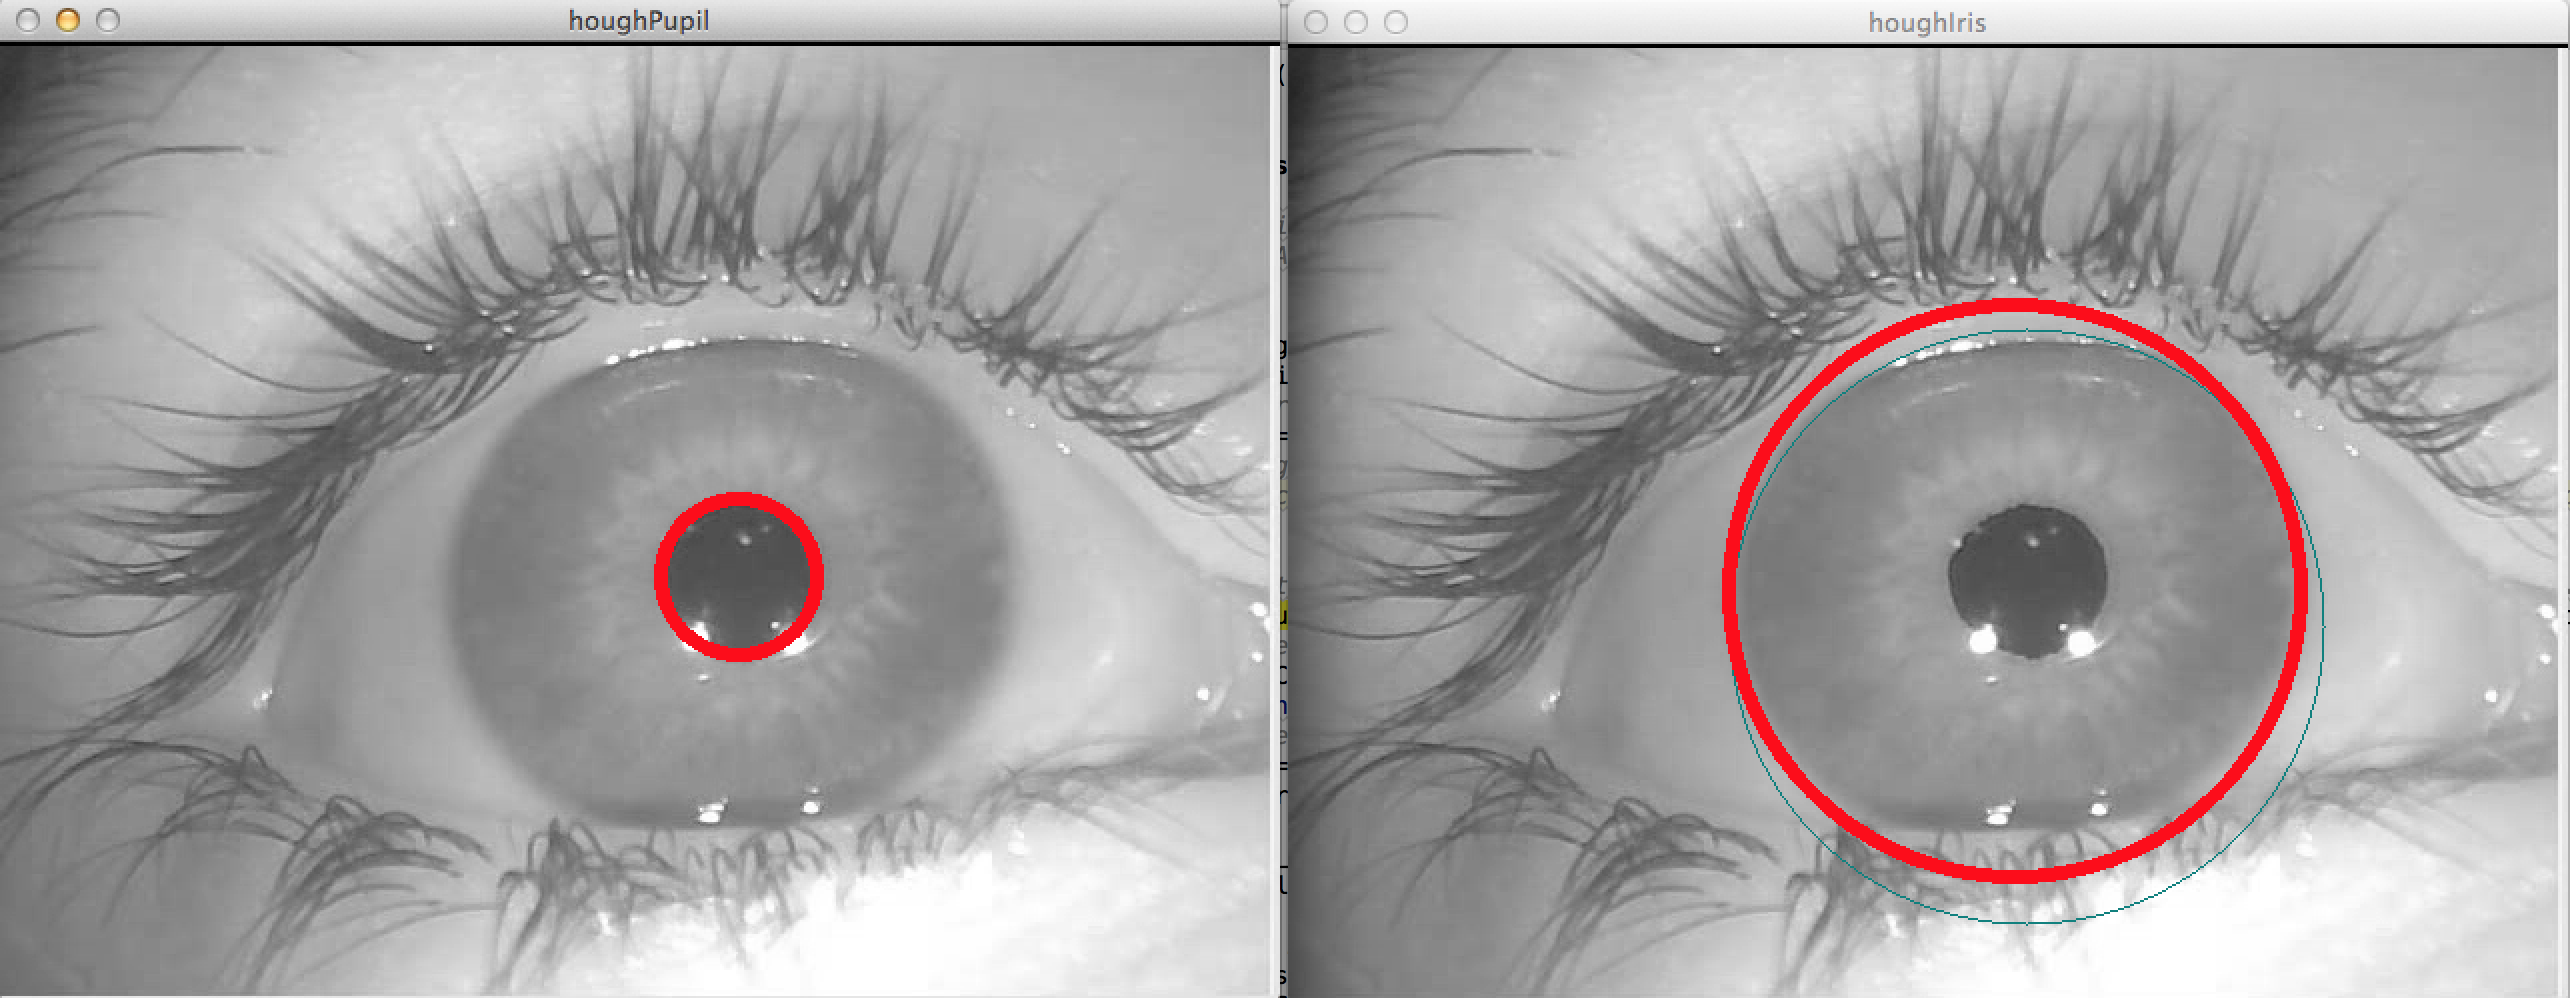
\includegraphics{pics/houghtransform.png}
\caption{Eye located with hough}
\end{figure}

\section{Pupil detection}

\subsection{Overall rationale and theory}

The eye consists of several distinct features such as pupil, iris,
limbus and sclera. Furthermore several features are present in images as
result of the light conditions when a picture is taken. The position of
these can aid in correctly determining the gaze. Detecting these
features is therefore a good starting for a gaze tracker implementation,
but it poses some challanges in correctly identifying each component,
and filtering away noise.

Of these features one of the easiest to recognize is the pupil, as it is
the darkest part of the eye. Furthermore it's good starting point, as it
is surrounded by the other eye components. The challenges/noise in
locating the pupil is mostly due to glints/reflections of light, but
these also aids in locating the pupil because we know that the pupil
will reflect light in a certain way.

As mentioned, the pupil is the darkest part of the eye. Furthermore a
pupil will reflect two ``glints'' of light. A good way to find the pupil
is to find an intensity value which can seperate it from the background.
This is called thresholding, and will be explained in the following
sections. Thesholding can be applied to both find pupil candidates as
well as glints used for more robustly picking the best pupil candidate.
When thresholding has been performed we will analyse certain features of
the BLOBs in the image to see which are good candidates for pupil and
glints. To aid in selected a proper threshold we will use a form of
pixel clasification to automatically set a threshold. This method will
be described last in this section.

\subsection{Thresholding}

Thresholding is a form of point processing used for seperating areas of
an image based on intensity in these areas. The desired end result of
this method is a binary image with the foreground (object) in one color
and the background (everything else) in a different color. This is
usually black and white respectively. This will effectively seperate the
foreground from the background for us, leaving us with only the
contours. In that sense we loose information and granularity in the
image, but since we're only interested in position we haven't lost
anything important.

\subsubsection{Theory}

As with all point processing methods the basic theory behind
thresholding is applying a calculation to every pixel in the image,
effectively changing the value of that pixel. We know that the end
result is a binary image, following this, each pixel will be transformed
into one of two values. We've so far operated on byte images so the max
value is 255 and the min value is of course 0. For clarity we will
assign each pixel either the min or the max value. Thus thresholding can
be expressed as the following with T being the assigned Threshold value
and f being the function applied to each pixel:

if f$(x,y) \leq T \quad then \, g$(x,y) = 0 \quad and \quad if
f$(x,y) < T \quad then \, g$(x,y) = 255

Performing these operations will leave us with an image where only
certain BLOBs are visible. We can then analyse the properties of these
BLOBs to find which one is most likely to be a pupil, and which are most
likely to be glints. Namely we will look at the area and the circularity
of blobs. Area is simply a count of all pixels in the blob.

Finding the circularity is a bit more complex. Used here is ``Heywoods
circularity factor'' which is derived from the perimeter and area of the
BLOB. Perimeter is the count of pixels on the rim of the contour. A
``cheaper'' approximation can be found by taking the perimeter of the
bounding box of a BLOB. The bounding box can be found simply by finding
the lowest and highest values of x and y respectively within a BLOB.

Once we have the perimeter and the area heywoods method can be applied.
It's defined as follows:

$Circularity = \frac {perimeter} {2 * \sqrt{\pi * area}}$

The area and circularity will be used to identify the best candidates

\subsubsection{Our implementation}

The usefulness of thresholding relies on having a total binary image
with the foreground easily distinguishable from the background. The
foreground is the pupil. The pupil is a dark circle-like object
surrounded by a lighter circle (the iris). So we're looking for a
threshold value that is lower than the surrounding iris. In an ideal
world the pupil in it's entirety will have only one intensity
throughout, and the ideal threshold value will be that. However, the
world is rarely so black and white (literally) and this also isn't the
case here. Although the pupil is the darkest spot it's not completely
dark. So a threshold value of 1 would be far to low in most
circumstances. It also requires very specialized lighting conditions to
achive a pupil with the same intensity throughout, so there is no
``silver bullet'' threshold value which will perfectly cover the entire
pupil.

What we're looking for is a value that is close enough to every part of
the pupil and far enough away from every part of the iris. The way of
finding this perfect value is mostly trial and error in this stage.
Luckily we had a slider to play around with when searching for this
value. For the thresholding itself, a built in cv2 method was used.

\begin{verbatim}
val,binI =cv2.threshold(gray, thr, 255, cv2.THRESH_BINARY_INV)
\end{verbatim}
Where:

gray is our (grayscale) image

thr is our selected threshold value

255 is the maximum value

the last argument is a constant indicating that output is a binary image

We quickly saw that a good value for most of the sequences floats around
100. An example of this can be seen in figure \ref{goodthr}:

\begin{figure}[htbp]
\centering
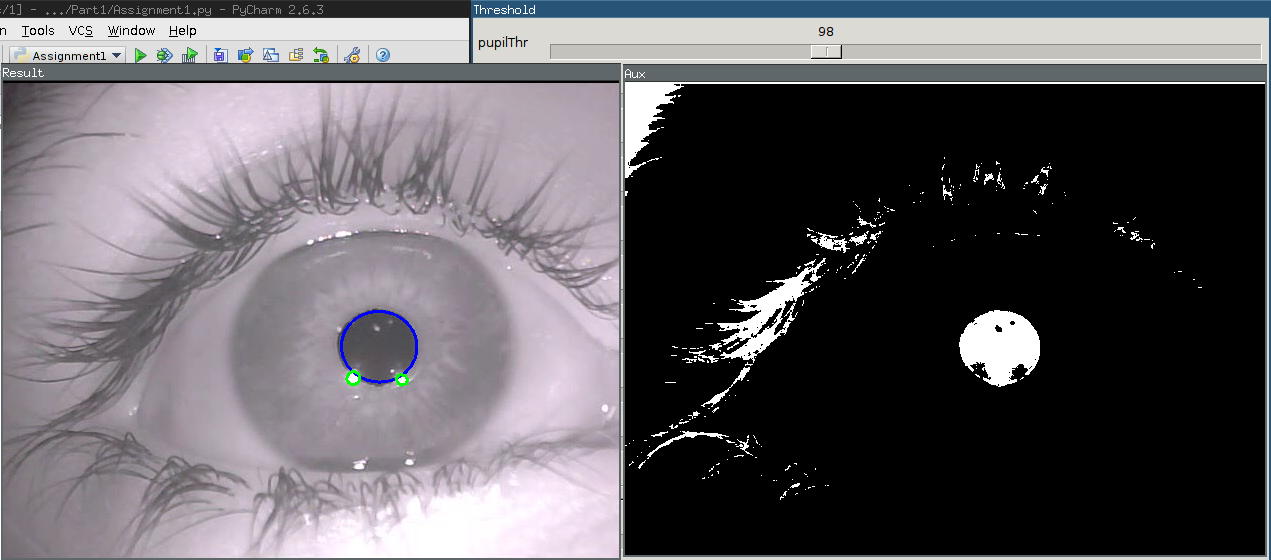
\includegraphics{pics/threshold_good.png}
\caption{Good threshold \label{goodthr}}
\end{figure}

This value is not robust in all cases, and too high or too low values
will yield to few or two many results respectively, seen in figures
\ref{lowthr} and \ref{highthr}

\begin{figure}[htbp]
\centering
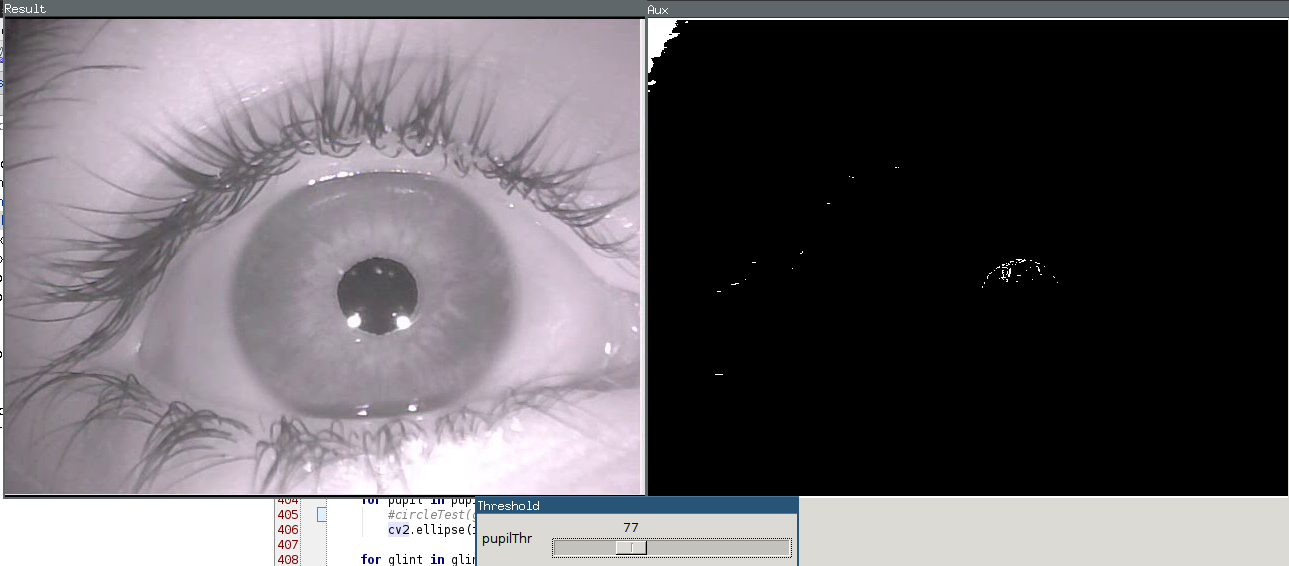
\includegraphics{pics/threshold_low.png}
\caption{Low threshold \label{lowthr}}
\end{figure}

\begin{figure}[htbp]
\centering
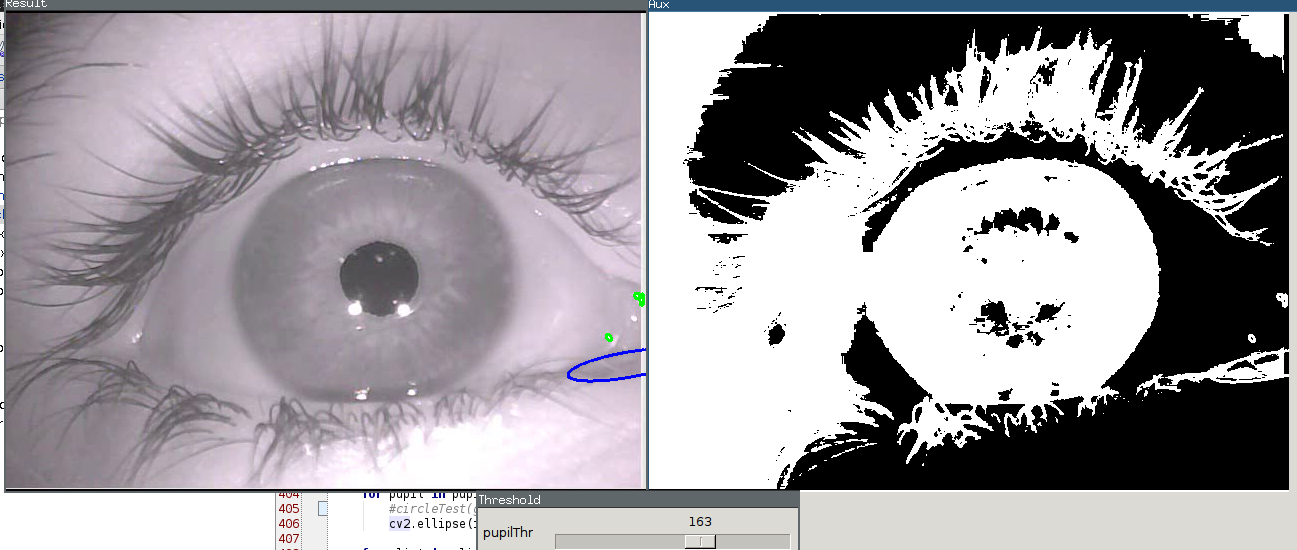
\includegraphics{pics/threshold_high.png}
\caption{High threshold \label{highthr}}
\end{figure}

Another aspect of this is that further analysis is needed on the
contours. So if a distorted figure is all we have it will be difficult
or impossible to correctly determine the nature of the contour. An
example of this false classification is seen in figure \ref{contourthr}

\begin{figure}[htbp]
\centering
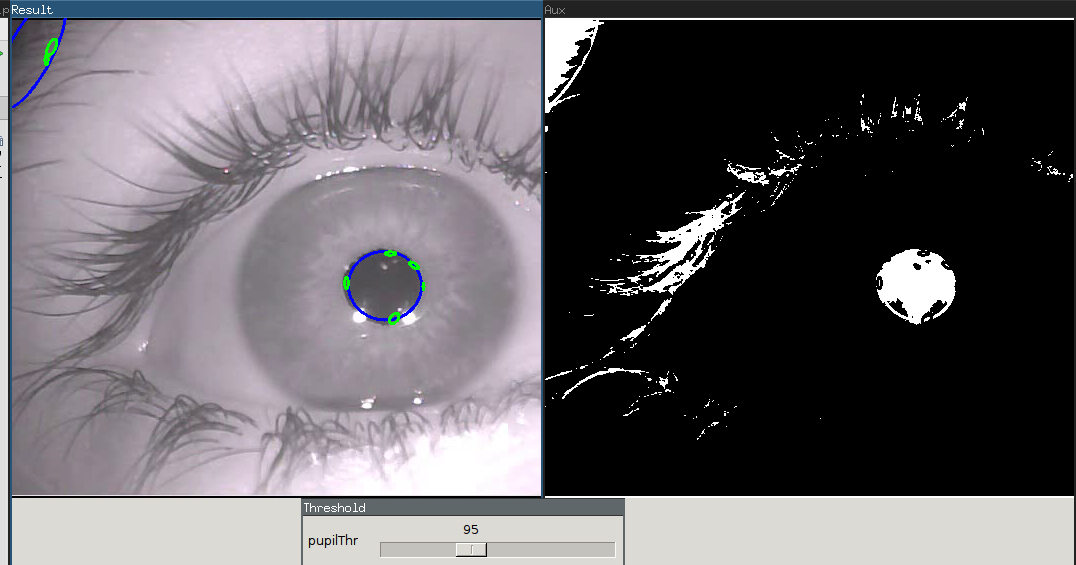
\includegraphics{pics/threshold_contours.png}
\caption{Contours found with threshold \label{contourthr}}
\end{figure}

In the happy path scenario analysis of the blobs will be performed as
described in the theory section above. First the area of the BLOB is
found:

This will be found using a cv2 methods. Presumably it's naively
implemented and has linear complexity, but this is speculation as we
don't have the implementation. Usage is as follows:

\begin{verbatim}
a = cv2.contourArea(con)
\end{verbatim}
Where con is a contour

Next the perimeters is found. Again opencv has an implementation for
this, given a closed contour:

\begin{verbatim}
p = cv2.arcLength(con, True)
\end{verbatim}
With these variables in hand the results can be filtered in a simple
imperative manner:

\begin{verbatim}
if(a==0 or a<minArea or a>maxArea):
    continue
p = cv2.arcLength(con, True)
m = p/(2.0*math.sqrt(math.pi * a))
if (m<1.7):
    if(len(con)>=5):
        ellips = cv2.fitEllipse(con)
        matches.append(ellips)
\end{verbatim}
The min and max area as well as the circularity value of 1.7 are found
through trial and error. The area parameters can be adjusted using
sliders as needed for each sequence. The constraints of the length of
the con is because we need 5 parameters for an ellipse

Last step is to redo this with the glints.

\begin{figure}[htbp]
\centering
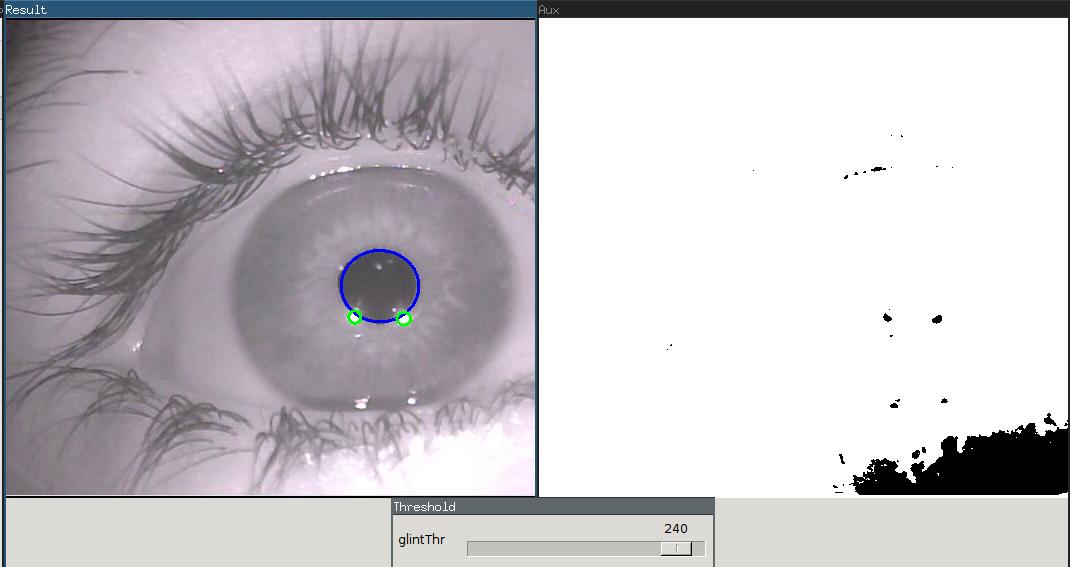
\includegraphics{pics/glintsthr.png}
\caption{Glints with threshold \label{glintsthr}}
\end{figure}

When we have the two glints of the pupil we can filter the data further
based on these newly found features. Out algorithm for this is very
straight forward and imperative:

\begin{verbatim}
for candA in glints:
    for candB in glints:
    #only accepting points with a certain distance to each other.
        if (Distance(candA[0],candB[0])> sliderVals['glintMinDist']
         and Distance(candA[0],candB[0]) < sliderVals['glintMaxDist']):
            glintList.append(candA)

#run through the remaining glints, keeping those that are 
#close to the pupil candidates.
for glintCand in glintList:
        for pupCand in pupils:
            if(Distance(glintCand[0],pupCand[0])>
            sliderVals['glint&pubMINDist'] and 
            Distance(glintCand[0],pupCand[0])<
            sliderVals['glint&pubMAXDist']):
                glintList1.append(glintCand)

#run through the pupil candidates keeping those that are close to 
#the fina glints list
for candP in pupils:
    for glintCand in glintList1:
        if(Distance(candP[0],glintCand[0])>
        sliderVals['glint&pubMINDist'] and 
        Distance(candP[0],glintCand[0])<
        sliderVals['glint&pubMAXDist']):
            pupilList.append(candP)

#sort out the pupils too far away from the found glints.
return (set(glintList1),set(pupilList))
\end{verbatim}
One critique of this approach could be that the pupil and glints depend
on each other ``both ways''. That is, we first filter the glint
candidates based on the pupil candidates and then the reverse is done.
However, the results seems to be fairly precise

\subsection{Pixel classification}

In this section it will be demonstrated how a form of machine learning
is applied to perform supervised classification in order to
semi-automatically set a correct thresholding value. Correct is defined
as a value which will allow us to perform the steps described in the
previous section

Clustering is the practice of grouping a set of elements into several
smaller groups of elements with similar features. It has a wide range of
applications within datamining and different types of analysis.
Obviously what will be demonstrated here is it's use within image
analysis. Clustering isn't a specific algorithm. Rather it's the task we
wish to perform in order to achieve our goal. In this assignment we've
used the k-means algorithm for this

K-means is a clustering algorithm which can group a number of
observations/data points into k number of clusters based on their
nearest mean value.

The properties of the k-means algorithm (k groups based on mean
intensity) combined with an existing knowledge of the properties of the
eye(the pupil is the darkest part) makes it possible to use k-means for
setting a threshold value automatically

\subsubsection{Theory}

The basic idea behind k-means clustering is to iteratively run through a
dataset assigning points in their correct cluster based on previously
selected values. Initially k points a selected and denoted as a center
for it's cluster, $c_1$ , \ldots{}, $c_k$ . These points can be selected
on random or based on some guessed distribution. On each run through the
dataset every points is examined. For each point the closest c is found,
and the point is marked as to belong to this cluster. Once all points
have been examined and placed in a cluster, the mean value of each
cluster is calculated as $c_ival$. Compare the mean value for the
cluster with the previously recorded value of $c_ival$. If it has
changed, another run through is performed. This continues until a
desired level of precision is achieved or amount of runs have taken
place

When we have done this we have k different threshold values to choose
from, given our knowledge of the pupil, we will choose the one with the
lowest mean value ($c_ival$).

\subsubsection{Our implementation}

There are a couple of possible caveats for this approach. Firstly there
is an element of uncertainty in exactly how the clusters will be
distributed. We need therefore to have a high enough k value to be sure
to get the right cluster. There is also some uncertainty about whether
the pupil always belongs to the darkest cluster. If for instance our
k-value is too high, and there exists a darker region in the image (dark
spot on the skin for instance) then the value of this cluster will be
chosen as a threshold value, and we might miss the pupil

Through trials it was found that 8 is a good value for k in the sense
that it often proved to segment the picture enough to allow the
intensity value of the pupil to exist in one of the clusters. The other
parameter is a constant that we apply so that the distance between the
points has less importance by dividing each point with this constant.
For this 15 was chosen as a good value.

The first step is performance optimization by resizing the image. This
saves a lot of computations:

\begin{verbatim}
smallI = cv2.resize(gray, reSize)
\end{verbatim}
where reSize is a 1x2 vector (30x30 was used)

When this is done we operate on column vectors

\begin{verbatim}
M,N = smallI.shape
X,Y = np.meshgrid(range(M),range(N))

z = smallI.flatten()
x = X.flatten()
y = Y.flatten()
O = len(x)
\end{verbatim}
From this we can create a ``feature'' matrix with values corresponding
to the intensity value of each pixel. Then the k-means algorithm is
applied to this feature-matrix to produce the centroids of each cluster.
The specifc k-means implementation comes from scipy. The same library
also provides a vector quantization which gives us the label for each
feature. Combining this we're left with a label image with intensities.
From these we pick the darkest and take that value as to mean the
intensity of the pupil. In reality this could probably be analysed
further to more robustly identify which cluster contains the pupil. For
instance we could analyse the original image and verify that there
exists an area with this intensity which looks sufficiently like a
pupil. If not, the second darkest area could be explored. This will
however further increase the computational complexity.

\begin{figure}[htbp]
\centering
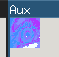
\includegraphics{pics/kmeans.png}
\caption{K-Means}
\end{figure}

\subsubsection{Usefulness of the k-Means algorithm}

K-Means seems very robust and definitely useful in applications like
this. A huge downside to this however is that it's computationally
expensive. Our implementation is at least. To overcome this we've used a
downsized image. As can be seen in figure \ref{kmeans}. This also makes
it very hard to visualize the method, as 30x30 pictures doesn't look to
great. If the downsizing isn't done, then the sequence can't really run.
One could argue that the lighting conditions of a picture rarely changes
on each frame. So doing k-means every time the frame is updated might be
overkill, and some calculations could be saved.


\section{Template Matching}

\subsection{What do we want to achieve?}

We want to describe how a succesful match is found for a template when
matching it with an image. We want to explain the main theories behind
the methods, and test our implementation under various circumstances.

\subsection{Main Theory: Use filtering methods}

\subsubsection{Correlation}

All the implementations of template matching (that we use) utilizes
variations of correlation, to compare templates with image segments. The
technique is the same as filtering with various predetermined kernels,
like gaussian, sobel, box-filter etc. , to gain various filter effects,
but instead we use an actual image template as a kernel and measure the
difference between this and a section of the image we want to look
through.

Normal (un-normalized) correlation is mathematically described as:

$h[m,n] = \sum{g[k,i] f[m+k,n+l]}$

Using this method for matching, is prone to a lot of ``false''
positives, as the result is dependent of the actual pixel values, not
determined by the degree of match between the filter and the image
segment. The sum of the multiplied pixel values, will be large in bright
areas of the image and vice versa in the dark areas. To make sure the
correlation also considers the overall brightness of the segment, a
normalized version of the formula is introduced.

If you step out one level of abstraction and view the template H and
image segment F as two vectors (achieved by joining each row or column
after each other), the correlation can be viewed as finding the dot
product between the two vectors. H dot F. (Just take a second and
realize that the dot product is found the same way as we calculate
correlation). As we know a vector can be normalized by dividing it by
its length, we can also normalize the dot product by dividing it by the
multiplication of the length of the two vectors.

the relationship is described in the formula:

$H \cdot F = ||H|| * ||F|| * \cos{V}$

\begin{center} 
$\leftrightarrow$
\end{center}

$\cos{V} = (H \cdot F) /(||H|| * ||F||)$

The normalised expression will always give a result between -1 and 1 as
$\cos{V} \exists [-1,1]$, and since the image vectors only contains
positive numbers the result will be betweem zero and one.

The length of each the two vectors are found with the formula: (here
with a vector in 3 dimensions)

$||a|| = \sqrt{a_1^2 + a_2^2 + a_3^2}$

Translating back from this abstraction level and looking at correlation
again the formula is translated into:

Normalized Cross Correlation:

$(x,y) = \sum{g[k,l] f[m+k,n+l]}$

This can be refined further by subtracting the means for both template
and image patch. This gives us the zero mean normalized
cross-correlation, AKA correlation coefficient:

\[h[m,n] = \frac{ \sum{k,l}{(g[k,l]-\bar{g})(f[m+k,n+l]-\bar{f}_{m,n})}}{((\sum{k,l}{g[k,l]-\bar{g})^2\sum{k,l}{(f[m+k,n+l]-\bar{f}_{m,n})^2)}^{0.5}}}\]

This gives a very accurate result, but is pretty slow as well.

\textbf{Another implementations using correlation:}

Sum of squared difference:

$d(u,v)=\sum{x,y}{f(x,y)-t(x-u,y-v)}^2$

This compares each corresponding pixels describing the difference
between them with a calculated positive number. (because of the squared)
The closer to zero the final result is, the better the match. The image
viewed (where white equals good results) are calculated with: image
(x,y) = 1 - sqrt(result of above expression).

Our Implementation is seen in figure \ref{getEyeCorners}

\begin{figure}[htbp]
\centering
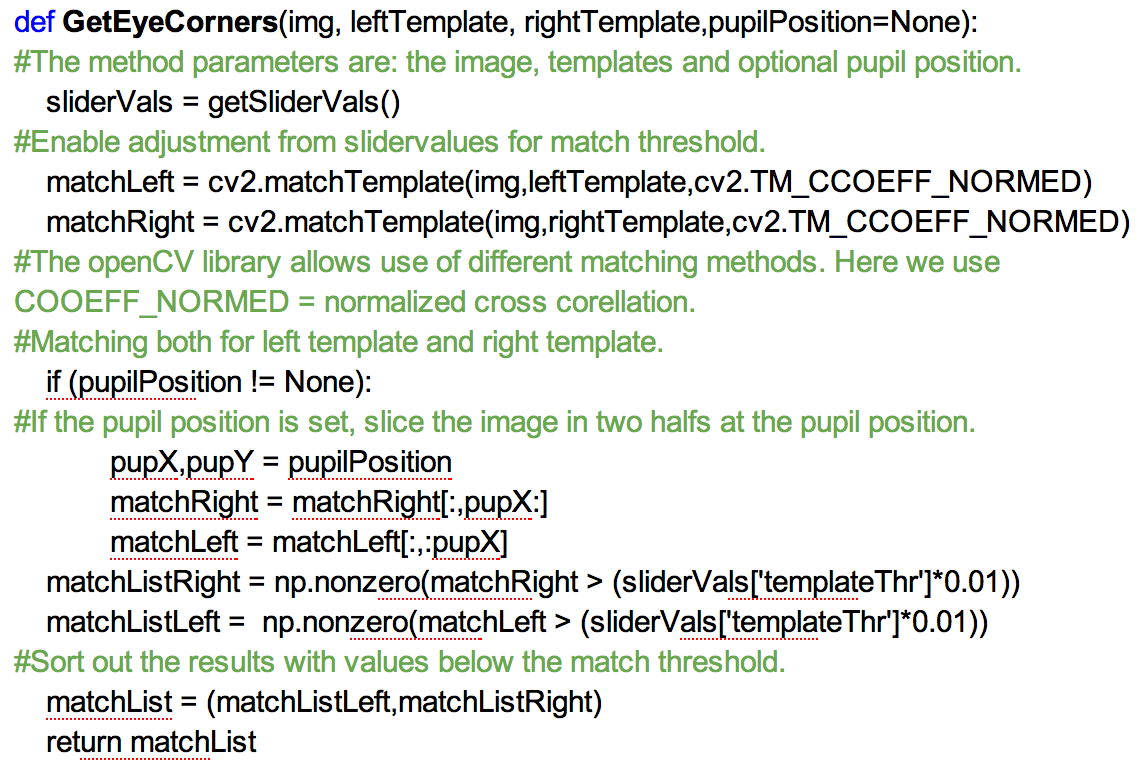
\includegraphics{pics/template_matching/getEye.png}
\caption{GetEyeCorners \label{getEyeCorners}}
\end{figure}

\pagebreak

\subsection{Our Results: (Also see video)}

We found that, when using the normalize cross corellation, a good
starting threshold is 0.85. That doesn't draw to many detections from
the start and, provides a good starting point for further adjustments.
All the tests runs utilizes the pupil position, allowing matches for the
left template only in the left side and opposite for the right template
matches.

\subsubsection{Test 1 - Unknown Subject.}

\begin{figure}[htbp]
\centering
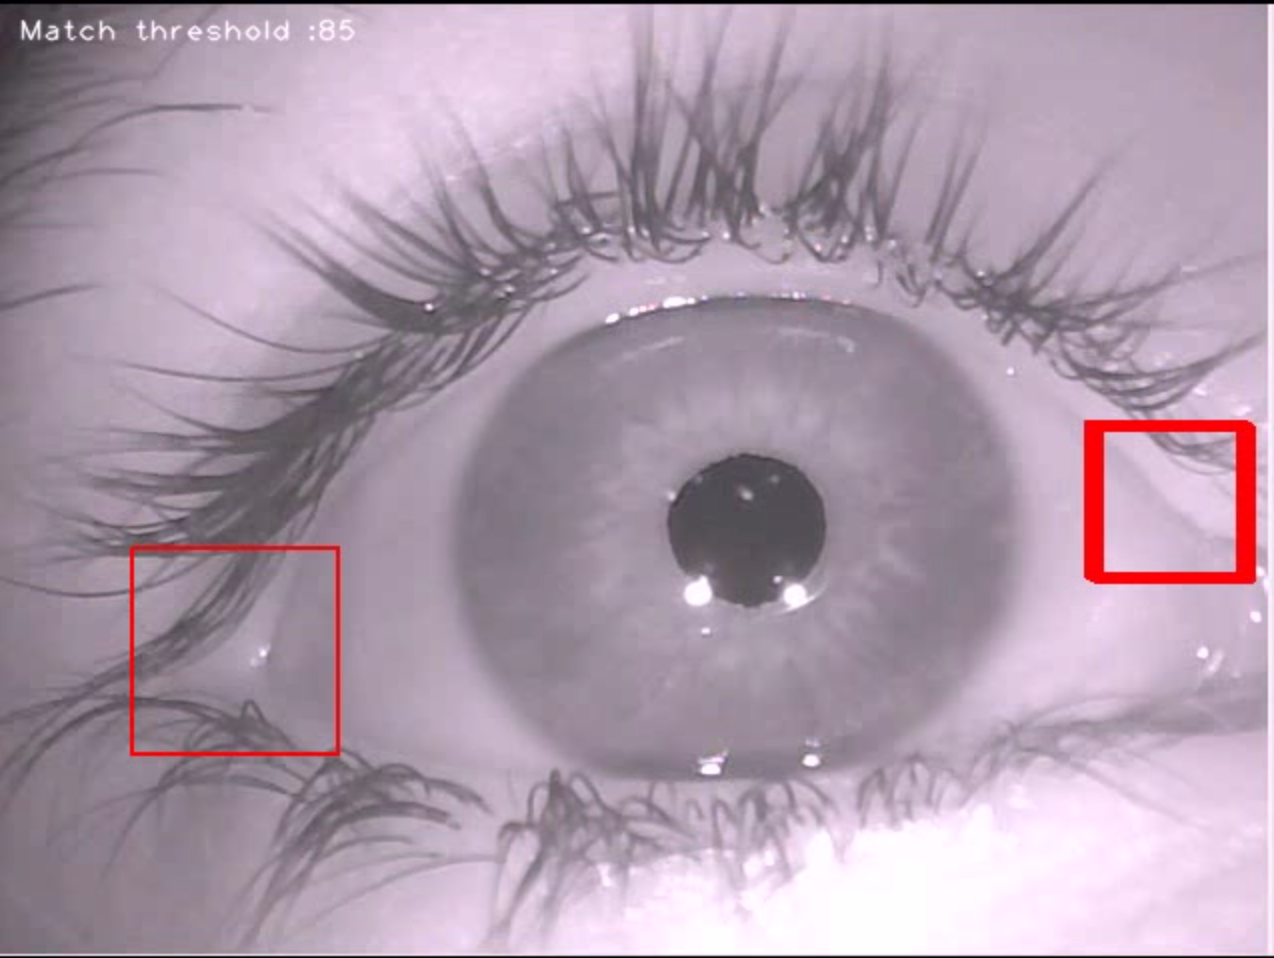
\includegraphics{pics/template_matching/1.png}
\caption{As we see in figure \ref{tm1}, with at threshold of 0.85,
things work out fine, when there are not too much movement in the image.
In controlled light, controlled subjects, the correlations methods works
like a charm. \label{tm1}}
\end{figure}

\begin{figure}[htbp]
\centering
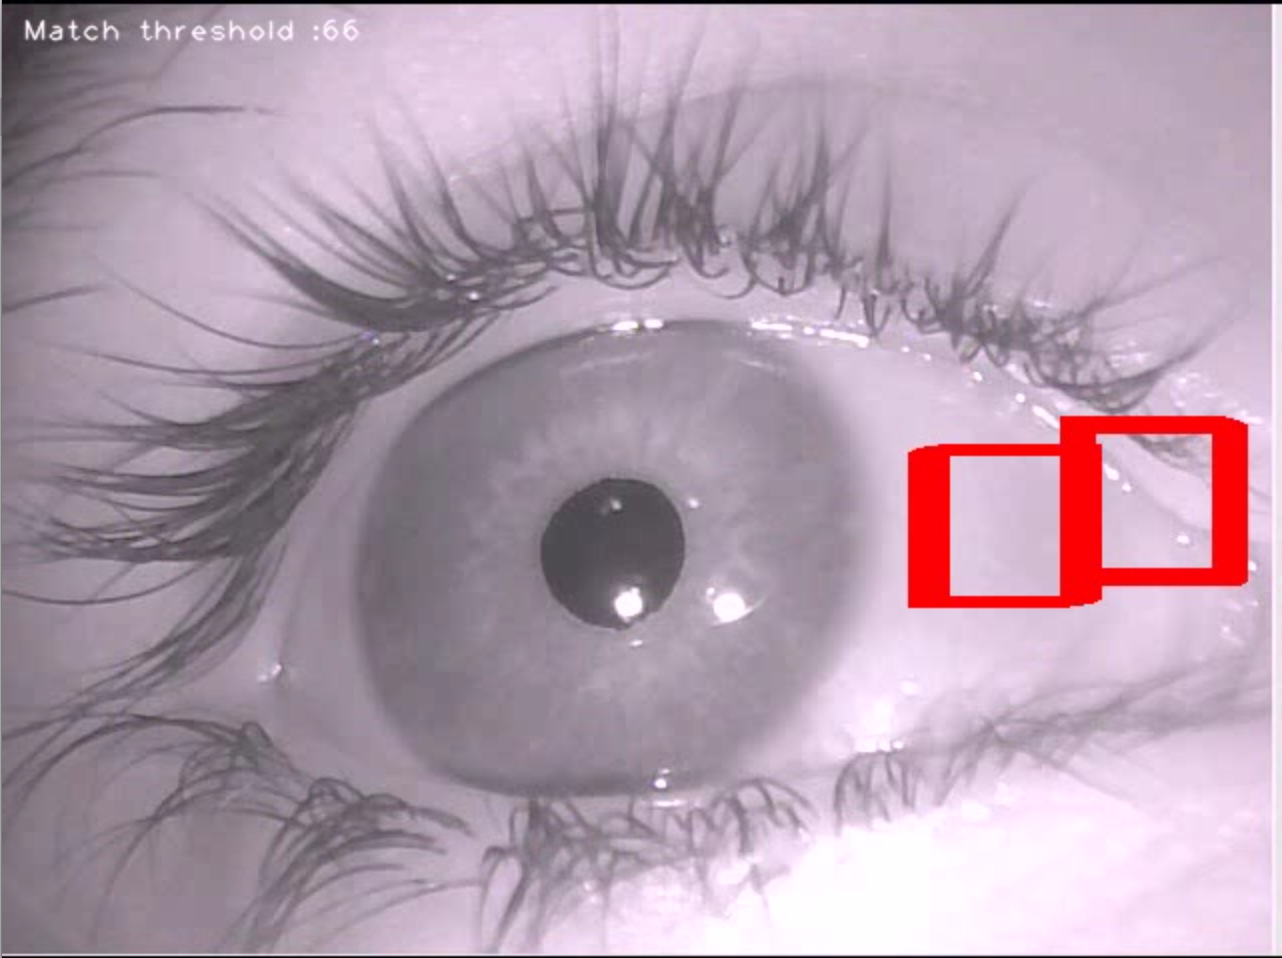
\includegraphics{pics/template_matching/2.png}
\caption{Seen in figure \ref{tm2}. As soon as the subject moves too
much, the threshold has to be lowered to find any results. It quickly
becomes a problem having a shared threshold for both template matchings
(left \& right), as the circumstances around the two places in the image
are quite different \label{tm2}}
\end{figure}

\begin{figure}[htbp]
\centering
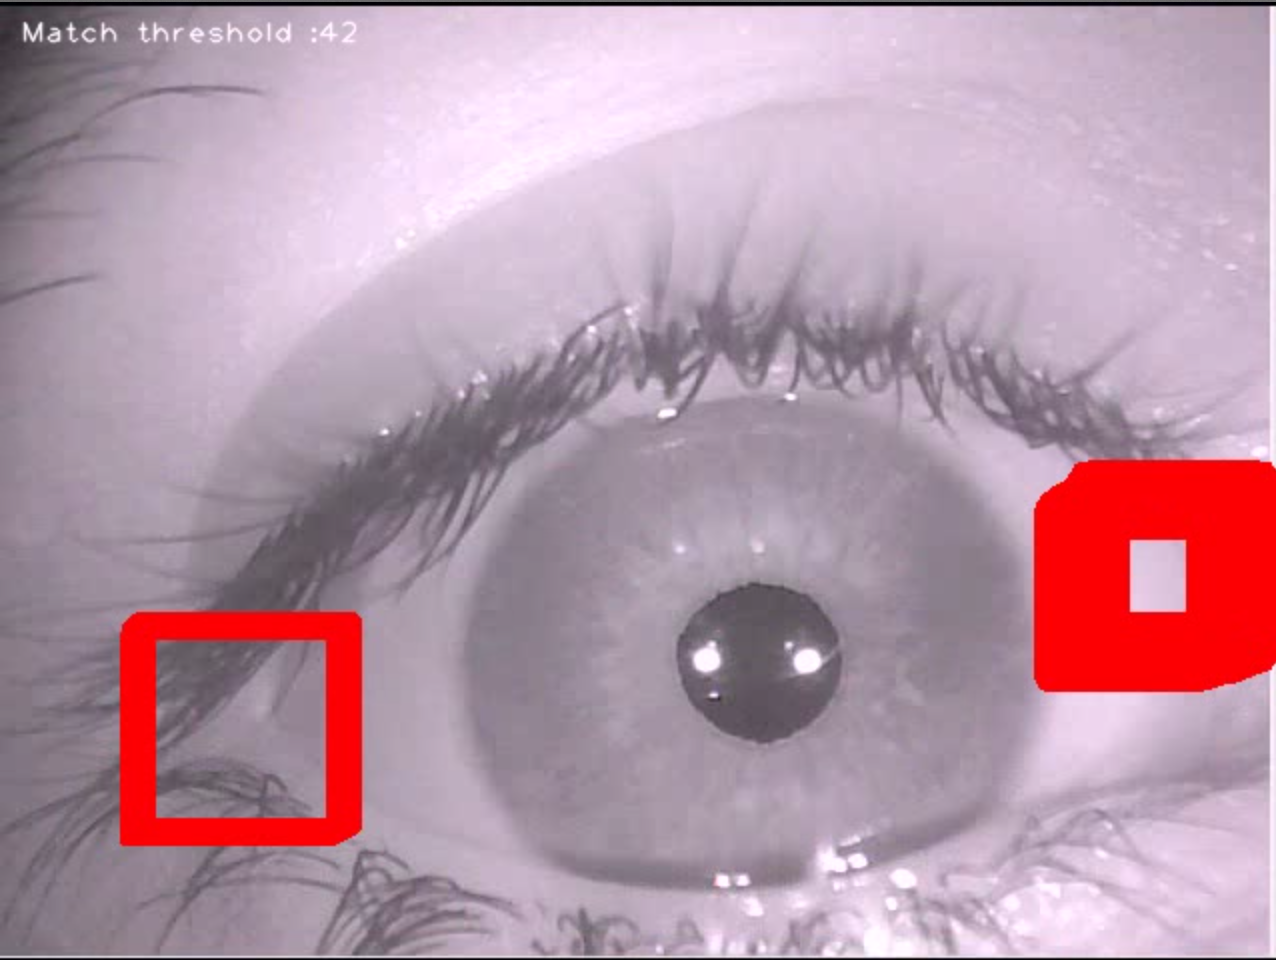
\includegraphics{pics/template_matching/3.png}
\caption{Seen in figure \ref{tm3}. Lowering the threshold even more,
allows the subject to move more freely and still finding matches in both
sides. Again we see a big difference in which sides that struggle and
which that finds multible matches. \label{tm3}}
\end{figure}

\subsubsection{Test 2 - Young Master Ghurt - recorded tuesday 12/03/13}

\begin{figure}[htbp]
\centering
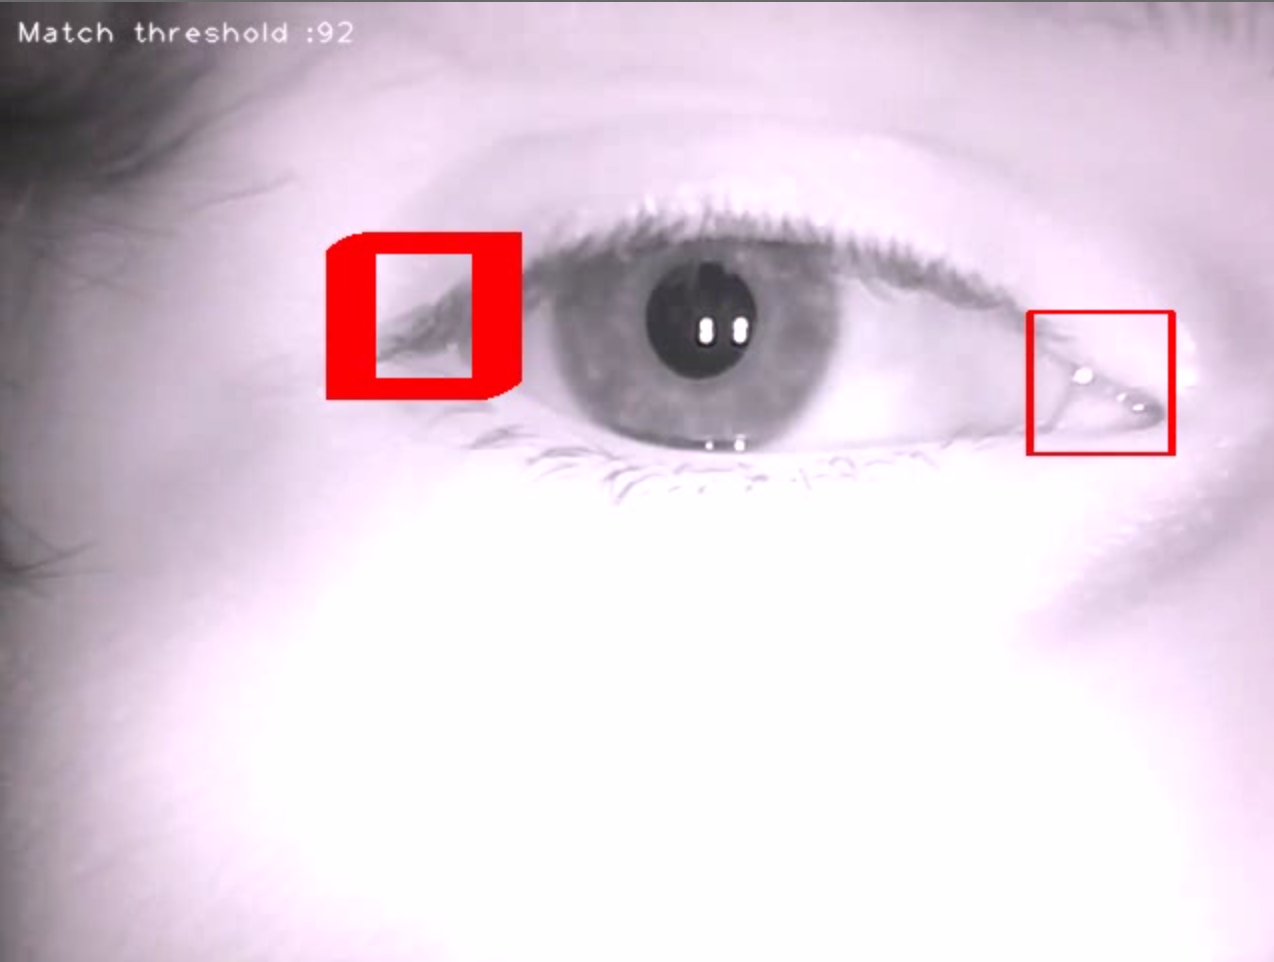
\includegraphics{pics/template_matching/4.png}
\caption{In figure \ref{tm4}. Starting out with a high threshold of 0.92
seems to work quite well. When the template contains enough
contrasts/diversity, and the subject remains still, the errors are few
\label{tm4}}
\end{figure}

\begin{figure}[htbp]
\centering
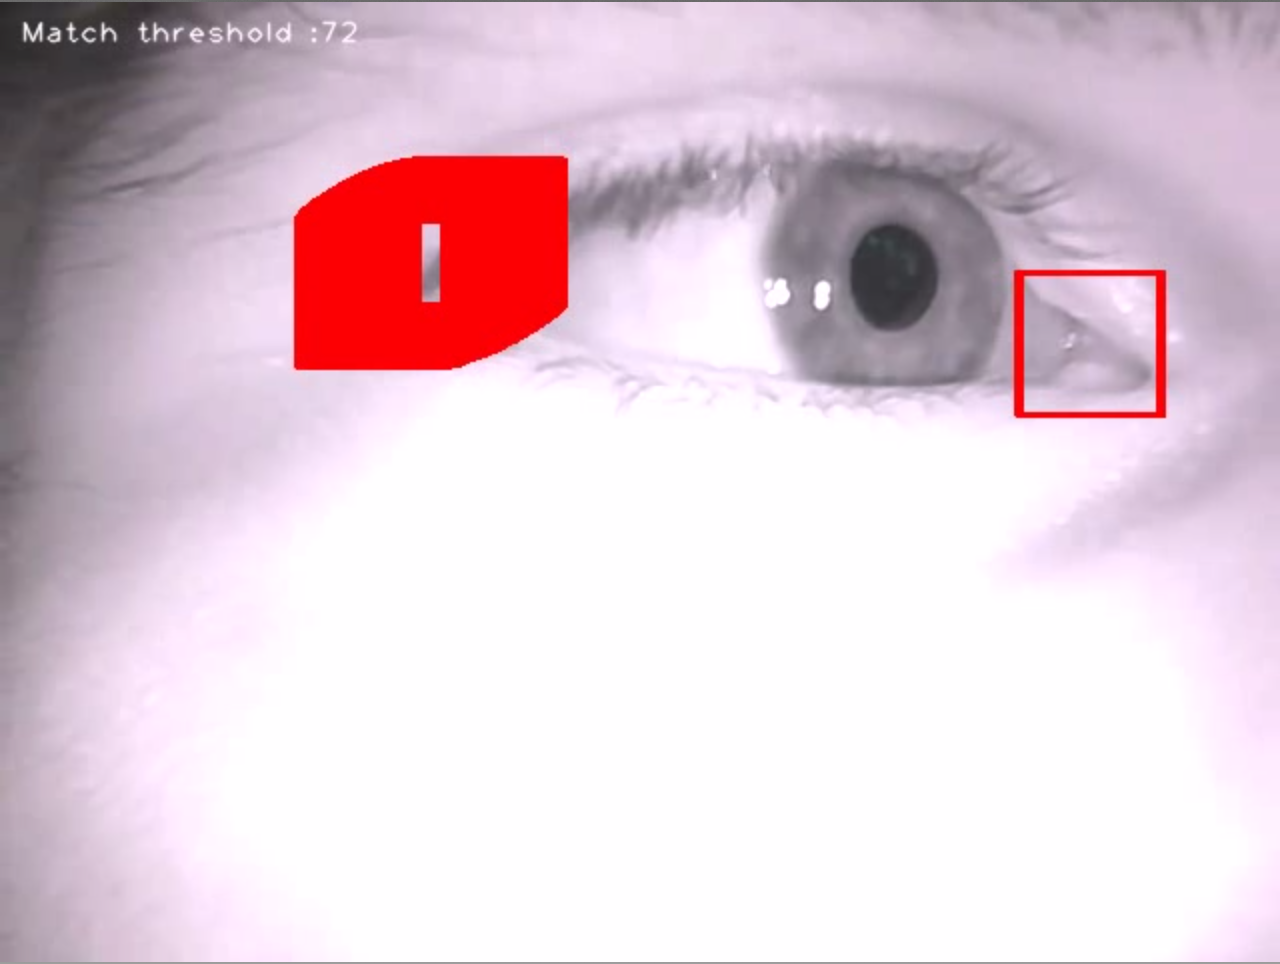
\includegraphics{pics/template_matching/5.png}
\caption{In figure \ref{tm5} we see it doesn't take a lot of change
before the threshold has to be lowered to find a result. Again there is
a huge difference on the sides, and we can conclude that a shared
threshold wouldn't be suitable in an industrial/finished solution.
\label{tm5}}
\end{figure}

\begin{figure}[htbp]
\centering
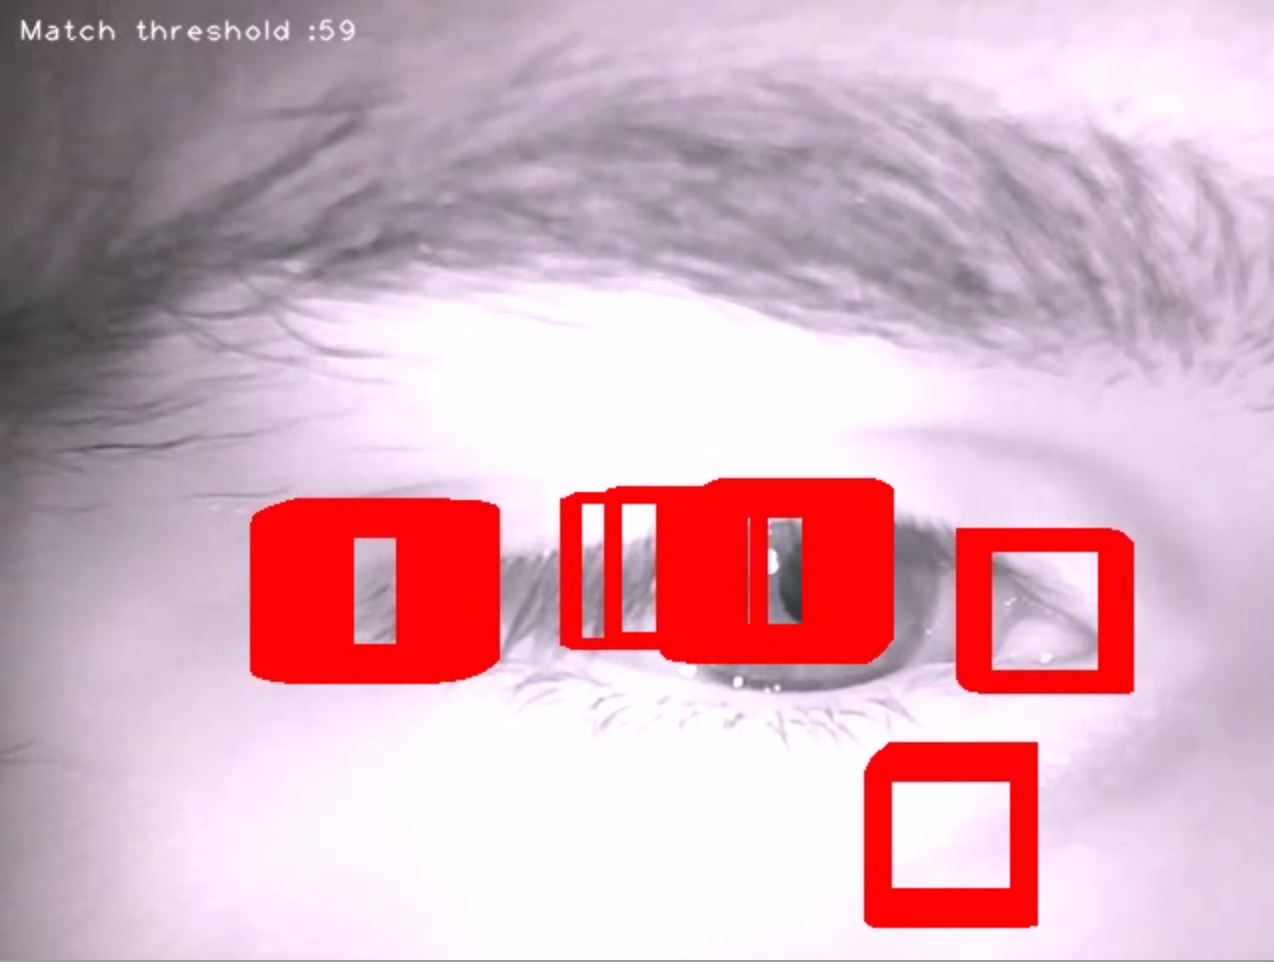
\includegraphics{pics/template_matching/6.png}
\caption{In figure \ref{tm6} we see as we continue the path downwards
lowering the threshold to find matches at the sides, a lot of false
results now appear, as the match no longer have to fit perfectly. This
is not a bad setup for further development, as the ``bad'' results
easily could be filtered away. (in the sense that too many matches are
better than none at all). \label{tm6}}
\end{figure}

\subsection{Concluding on the results and improving the method:}

It is obvious that our implementation can be improved. As in all the
different techniques mentioned in this report, controlling the
circumstances are vital for success. Out of the box, cross correlation
proves to be a pretty solid way of finding matches, but it requires the
subject to stand still and keep the same angle towards the camera so the
match area doesn't change completely. The method doesn't provide blazing
speeds as it is now. But this could be improved by performing some of
the work in parallel processes. Instead of matching twice with different
templates, you could use one common template, that would find enough
matches on each side and then filter out bad reslts even more. As of
now, results for are only restricted in that they have to appear on the
correct side of a found pupil location. This could be even more
improved, utilizing the distance from each other, or placement relative
to other facial features. As with the other techniques it proves
impossible to find parameters to fit a sequence of images where the
subject changes/moves. It's far better to find many matches and the
remove ``bad'' results afterwards.


\pagebreak
\section{Edges and Gradients}
\subsection{Overall rationale and theory}
Extending on the previously described means of detecting the pupil, image
intensity gradients provide a method for finding the edge between pupil and
iris, as well as the limbus (the edge between iris and sclera).The problem of
finding edges in an image can be reduced to the problem of finding high
magnitudes in the image's gradients.
In practice:
\begin{itemize}
	\item Noise reduction is performed,
	\item The image gradients are found, and
	\item A subset of the gradients are scanned to determine the location of edges in the
original image.
\end{itemize}

\begin{figure}[htbp]
%\centering
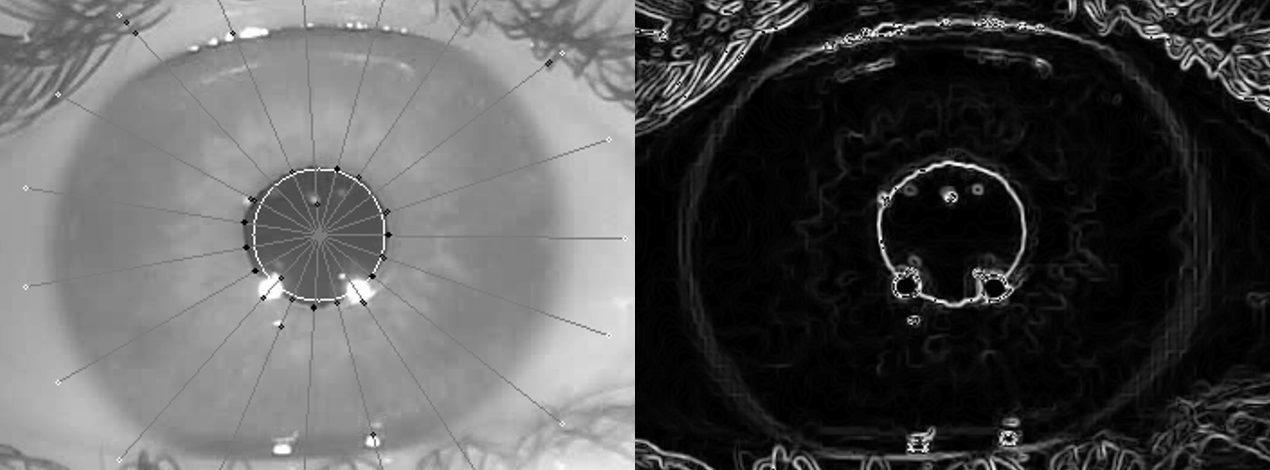
\includegraphics{pics/normallines_with_maxima_vs_gradient.png}
\caption{\textbf{Left:} Black dots are the highest gradient magnitudes found on the grey
lines (here, 2 per line). The white circle is the initial estimate of the
pupils location. \textbf{Right:} The set of gradient magnitudes represented as an image.}
\end{figure}

\subsubsection{Using gradient magnitudes}
A bilateral filter was chosen for noise reduction. In contrast to blurs like
gaussian filters, bilateral filters weigh the inputs according to both
euclidean distance to the output pixel, and the intensities in the source
patch. The consideration of intensity differences makes bilateral filters edge
preserving which, not surprisingly, is crucial for edge detection.

The image gradients are found by applying the sobel operator on the image. In
effect; finding approximated partial derivatives for the vertical and
horizontal axes respectively. Together, the two derived images form a set of
vectors, each describing the gradient for its pixel location. The length of one
of these vectors is the gradient magnitude of a certain point in the original
image. That is; the rate of change in intensity in a specific pixel. An
''edge'' is a continuous path of high gradient magnitudes. The gradient
magnitude in the point $(i,j)$ is found by $$\sqrt{x^2+y^2}$$ where $$x =
\frac{\delta z}{\delta i}, \quad y = \frac{\delta z}{\delta j}$$ and $z$
denotes pixel intensity. The scanned lines are chosen as the normals of a
previously found estimate of pupil, here scaled to 4.5 times the estimate’s
radius, and spaced with 0.314 radians. In principle this method should provide
20 points on the periphery of the pupil, and should be extensible to finding
the limbus. In practice, however, a few problems might arise.

\subsubsection{Using gradient orientation}
When examining the above two images of the eye, it becomes obvious that the
pupils edge might not be have the highest gradient magnitude. For example, the
eyelashes and glints might give a larger intensity change, than the
black-to-grey change between pupil and iris.Luckily this problem can be
bettered using information already available, namely the image gradients’
orientations. By considering the gradient’s angle to the pupil normal, some of
the high gradients can be discarded. This works on the assumption that the
pupil is fairly circular, and that estimated pupil location is somewhat
correct. Thus, the angle between normal and gradient on the pupil edge will be
small.The gradients’ angles to the positive x-axis is found and compared to the
normals angle to the positive x-axis. The angle between a vector and the
positive x-axis can be found by applying the arctangens2 operator to its
lengths: atan2$(x,y)$.

The use of gradient orientation presents a new problem; performance. The use of
the atan2 operator proves to be heavy enough that it became necessary to reduce
the size of the input image. As this method assumes a previous estimate of the
pupil’s location, it might be preferable to select an image patch around the
eye, rather than actually downsampling the input image. Though the latter will
be less robust to change in eye size or distance to the camera. The described
method is applicable to limbus detection, but in practice the iris is much
harder to detect. This is probably due to the smaller contrast between iris and
sclera, as well as to the edge between them being ‘jagged’ (this is most
visible in the right side of iris in the above gradient image).

%In the current
%configuration, the provided code does not do limbus detection as it turns out
%to require a lot of tweaking.The theory applied should, however, be applicable
%for limbus detection.


\section{Hough Transformation}

\subsection{Main Theory:}

Hough transform is a voting technique that is used to determine the
``most possible'' lines in the image.

Each line in a 2d image can be represented by:

$y=mx+b,$ where (x,y) is a point in the image space.

Each line in image space can also be represented by a point (m,b) in the
Hough space, where:

$b = -mx + Y$

A single point (x,y) in image space maps to all solutions of
$b = -mx + y$ which corresponds to a line in the hough space.

\begin{figure}[htbp]
\centering
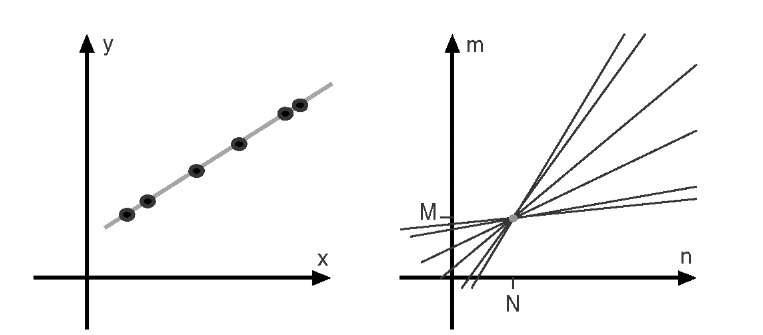
\includegraphics{pics/hough/1.jpg}
\caption{Hough space \label{hough1}}
\end{figure}

If we have two points (x0, y0) and (x1, y1) they'll each correspond to
lines in the hough space. As each point in hough space is a line in the
image space, the point where the lines intersect in hough space, will be
the line in the image space, that contains both points (x0, y0) and (x1,
y1). The solution to:

$b = -mX0 + y0$ and $b = -mx1 + y1$ (intersection between)

\subsubsection{How does it work?}

As input to a Hough algorithm we use a thresholded gradient magnitude
image. (see Fig. \ref{hough3}) This is usually computed by first doing
some soft smoothing, then using a Sobel filter (fig. \ref{hough2}) for
both vertical and horizontal directions.

\begin{figure}[htbp]
\centering
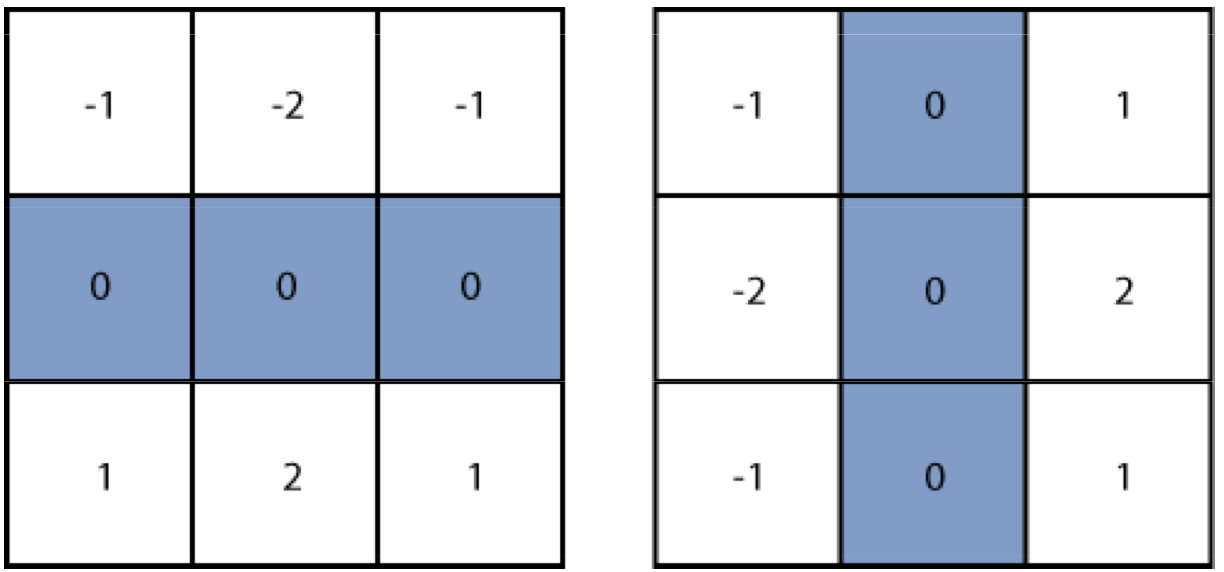
\includegraphics{pics/hough/2.png}
\caption{Sobel kernel \label{hough2}}
\end{figure}

From this image the edge magnitude image is computed, where:

$g(x,y)= sqrt(g2(x,y)+g2(x,y)) is the gradient norm for/in the point (x,y)$

\begin{figure}[htbp]
\centering
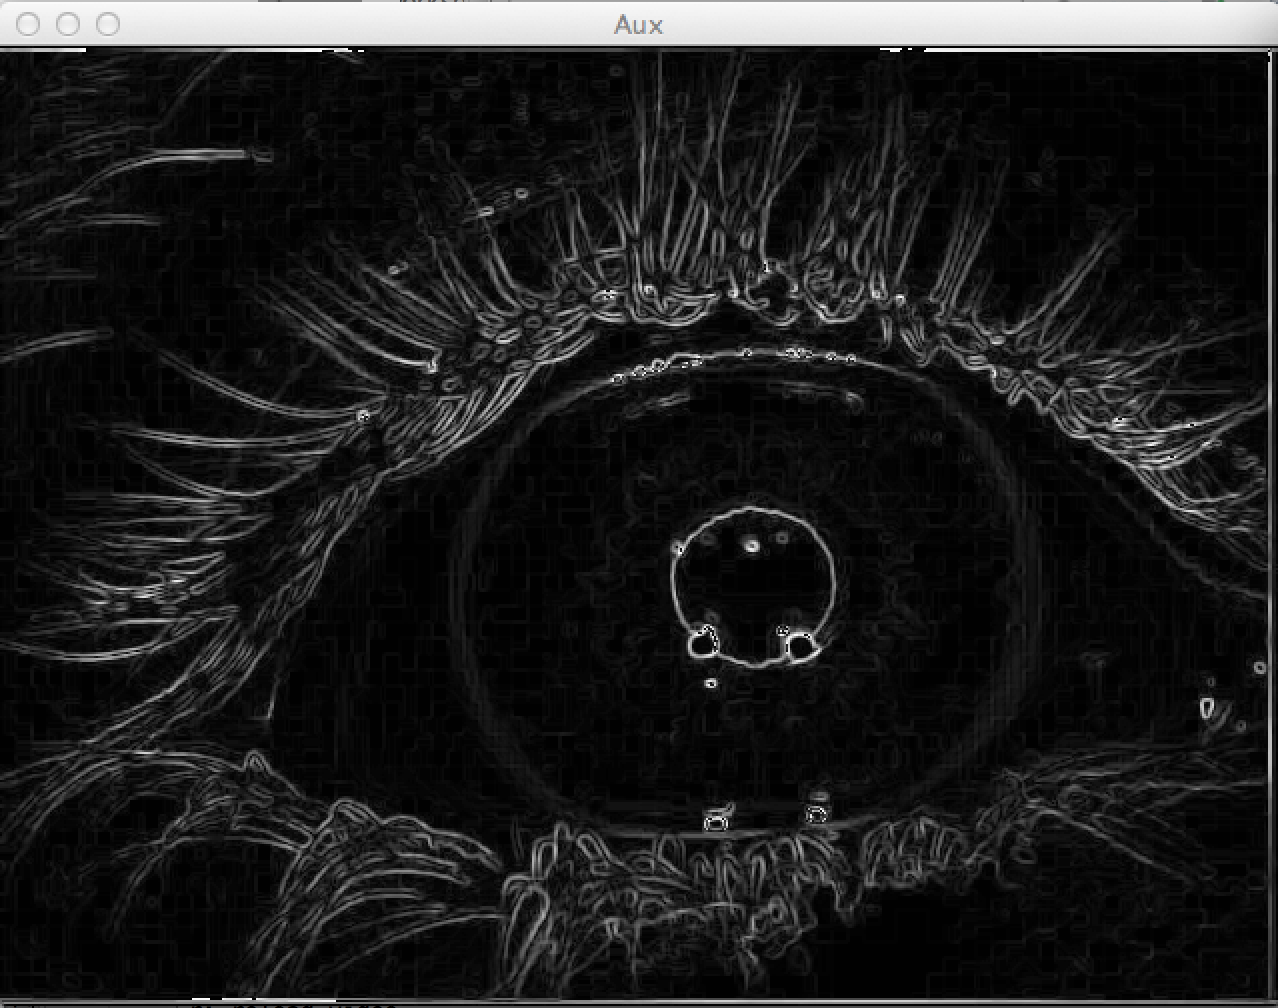
\includegraphics{pics/hough/3.png}
\caption{Our calculated edge magnitude image for a closeup image of an
eye. Brighter spots equals a longer gradient which means a larger
contrast \label{hough3}}
\end{figure}

Thresholding this image will (if we exclude all below the threshold)
give us a set of n pixels, that with high probability is part of a
edge/line in the image. Each of these pixels will produce an infinite
amount of lines in the Hough space. Where a lot of these lines intersect
is a point corresponding to a line in the image space. Each point in
image space, will produce a lot of ``bad'' results, and to filter out
these results the hough algorithm uses a voting system.

\begin{figure}[htbp]
\centering
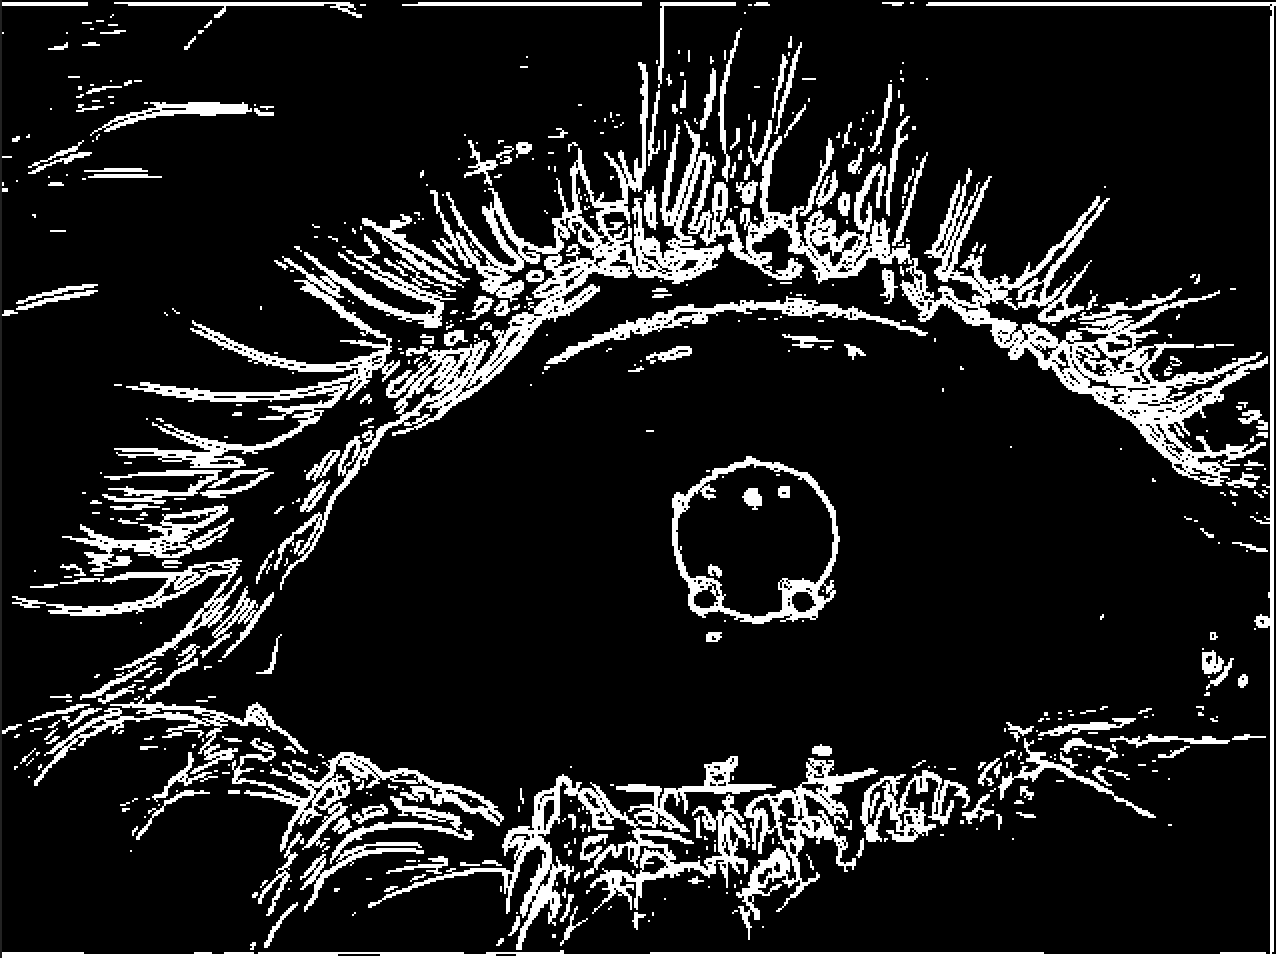
\includegraphics{pics/hough/4.png}
\caption{Thresholded magnitude image \label{hough4}}
\end{figure}

The hough space is quantized into small cells. Each time a line in the
hough space passes through a cell, the value of the cell is increased by
one. We say that the line ``votes'' for that cell. After calculating all
possible votes in the hough space, we'll end up with an accumulated
image, where several points have voted for certain points, thereby
voting for the existence of a line in the image space.

\begin{figure}[htbp]
\centering
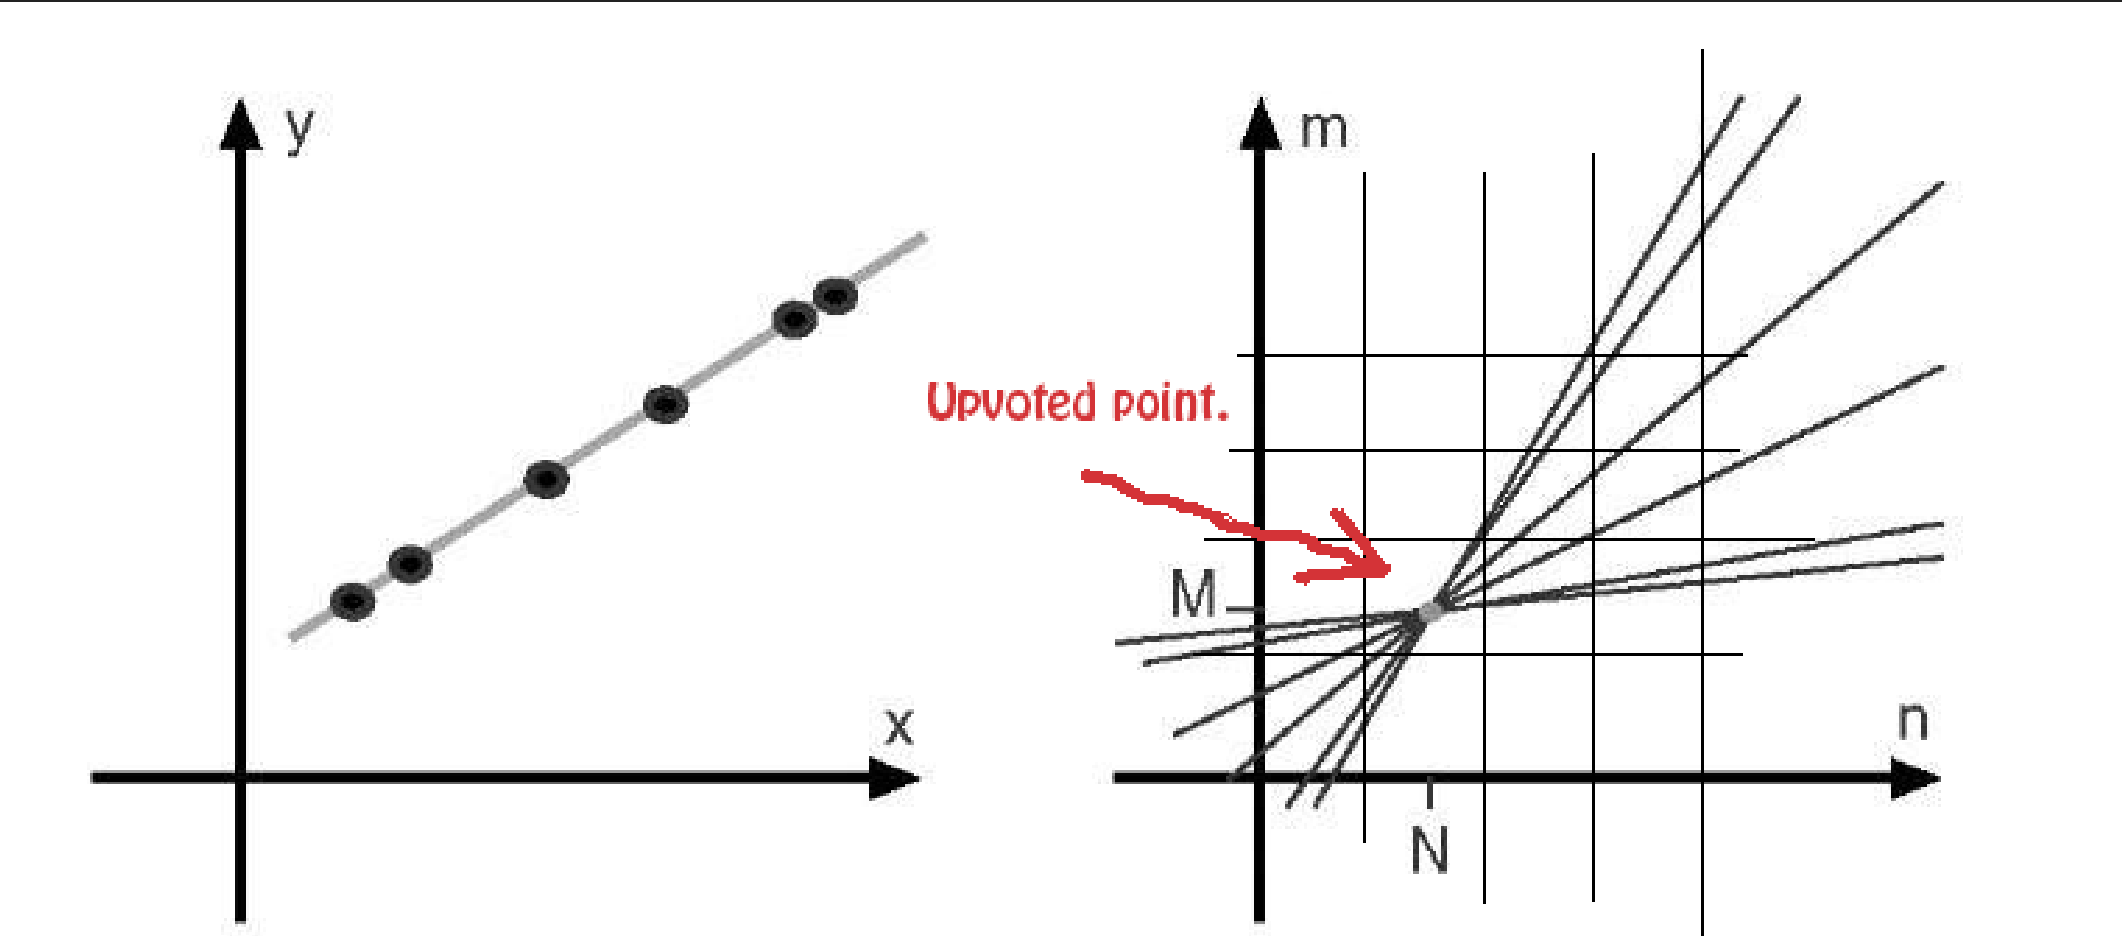
\includegraphics{pics/hough/5.png}
\caption{Upvoted point \label{hough5}}
\end{figure}

\subsection{Polar representation}

Using $b = -mx +y$ as representation in Hough space can be problematic
when dealing with vertical lines, so instead we use the polar
representation where each point in image space (x,y) corresponds to
points on the sinusoid curve
$x_i \cos{ \theta } + y_i \sin{ \theta } = \rho$ in Hough space. The
technique is the same, where each point $( \rho, \theta)$ on the curve
will up-vote points in the accumulated Hough-image $H[ \rho , \theta]$

\begin{figure}[htbp]
\centering
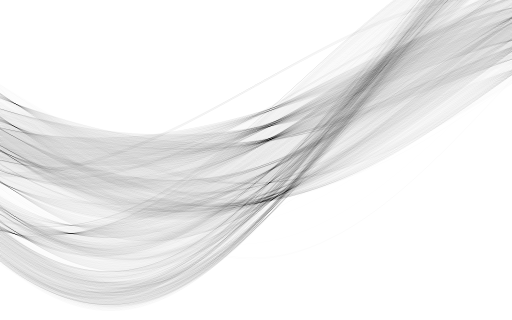
\includegraphics{pics/hough/6.png}
\caption{Hough space sinusoid curve. (Here rather illustrative but alas
not very informative, as it is without coordinates.) \label{hough6}}
\end{figure}

\subsection{Hough Circle Transform:}

In the line detection case, a line was defined by two parameters. In the
circle case, we need three parameters to define a circle.(From OpenCV
documentation.)

$C: (Xcenter, Ycenter, radius)$

The hough-space is therefore also increased by one dimension, to
accommodate the third ``unknown''. Should we wish to find more
sophisticated shapes, the hough space can theoretically be increased by
n dimensions. Although the calculations performed in the voting
algorithm, are expensive and the accumulated cost rise dramatically with
each dimension added.

\textbf{Open CV implementation:}

The openCV method first performs a canny edge detection, and then uses a
bit more complex voting method using the gradient directions to guide
the Hough voting process. (Presumably using the methods we described
earlier , sorting out voting results, where the angle between the
gradient, and the circle normal within a defined threshold. Although the
OpenCv documentation is not quite clear on this point).

\textbf{Our Implementation:}

\begin{verbatim}
def detectPupilHough(gray):
    #The method takes a gray-scale image.
        blur = cv2.GaussianBlur(gray, (81,81), 11)
    #The image is blurred to remove noise, that could potentially create gradiants where there are no edge. Its a fine line though, as the blurring potentially could make it harder to find the edges we're trying to locate.
        slidervals = getSliderVals()
    #This is so we can adjust the min/max radius for accepted circles.
        dp = 6; minDist = 30
    #This determines the resolution of the Hough-space and the minimum distance between found circles.
        highThr = 20
    #As the Cv2 uses canny edge detection, this sets the threshold for accepting “line” pixels.
        accThr = 150;
    #Determins how many votes that a circle should receive to be accepted (and drawn).
        minRadius = slidervals['Hough pupil size']-7;
        maxRadius = slidervals['Hough pupil size']+7;
    #Sets the size of the accepted circles.
        circles = cv2.HoughCircles(blur,cv2.cv.CV_HOUGH_GRADIENT, dp,minDist,                 None, highThr,accThr,minRadius, maxRadius)
    #The actual cv2 method that uses all the parameters just explained.
    #The rest is just drawing the circles (drawing a red circle for the circle with most votes.)
        gColor = cv2.cvtColor(gray, cv2.COLOR_GRAY2BGR)
        if (circles !=None):
                all_circles = circles[0]
                M,N = all_circles.shape
                k=1
                for c in all_circles:
                cv2.circle(gColor, (int(c[0]),int(c[1])),c[2], (int(k*255/M),k*128,0))
                K=k+1
                        c=all_circles[0,:]
                        cv2.circle(gColor, (int(c[0]),int(c[1])),c[2], (0,0,255),5)
cv2.imshow("houghPupil",gColor)
\end{verbatim}
\subsection{Our Results}

Finding the pupil: As with all the methods in this report, the
parameters of the cv2 method had to be adjusted to fit the resolution
and lighting of each video.

\subsubsection{Test 1. Unknown subject closeup.}

figure \ref{hough7} Test settings: Smoothing: gaussian blur, kernel size
(11,11). Circle Threshold: 200.

\begin{figure}[htbp]
\centering
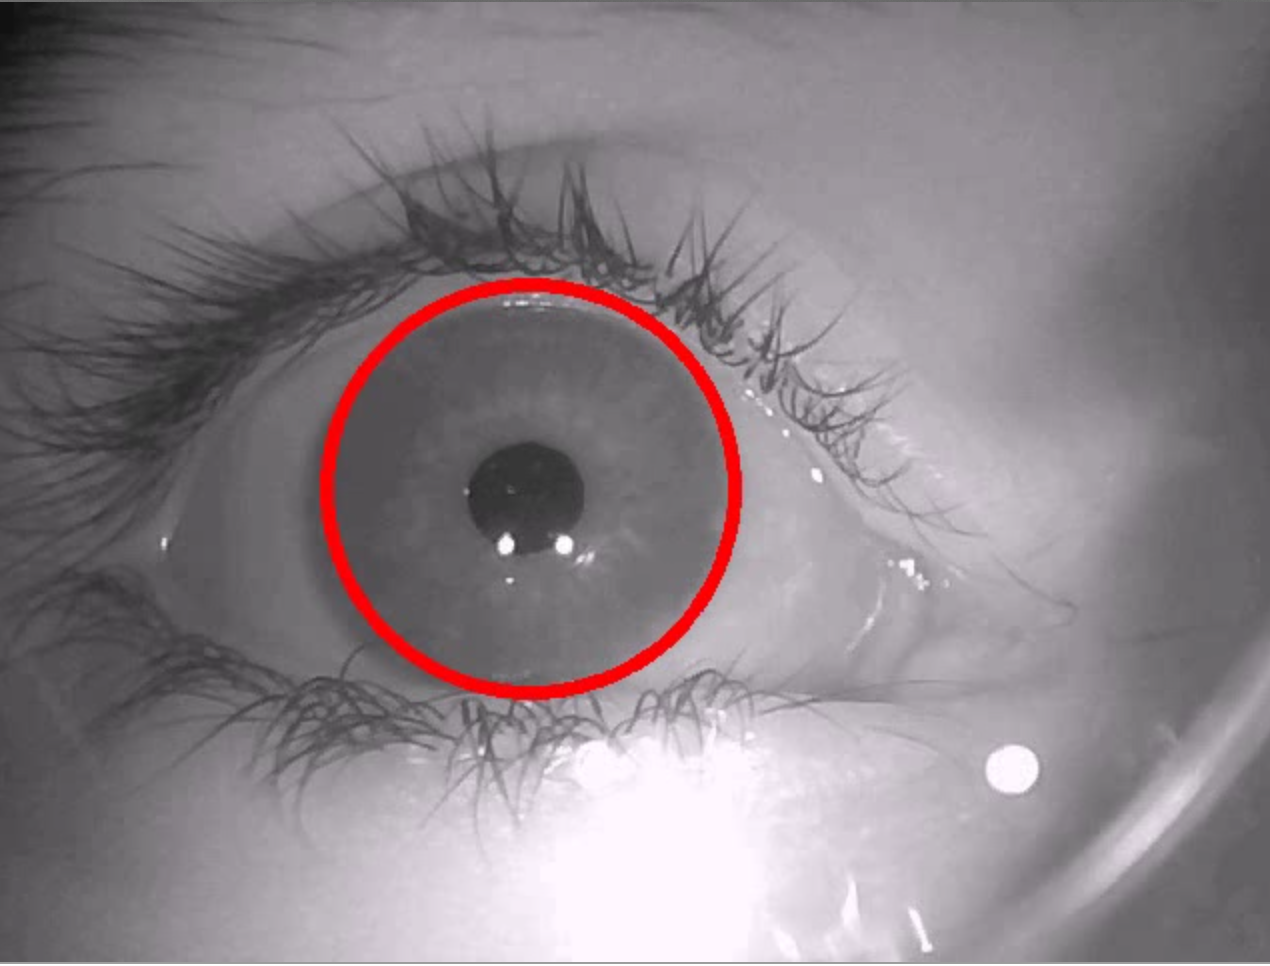
\includegraphics{pics/hough/7.png}
\caption{These circumstances are ideal for detecting the iris, as the
iris itself is highly visible and a lot of high contrast circle poins
help determine the circle placement. The top of the circle may be
detected on the eyelid rather than the iris though, as the contrast
there is larger that on the actual iris. \label{hough7}}
\end{figure}

\begin{figure}[htbp]
\centering
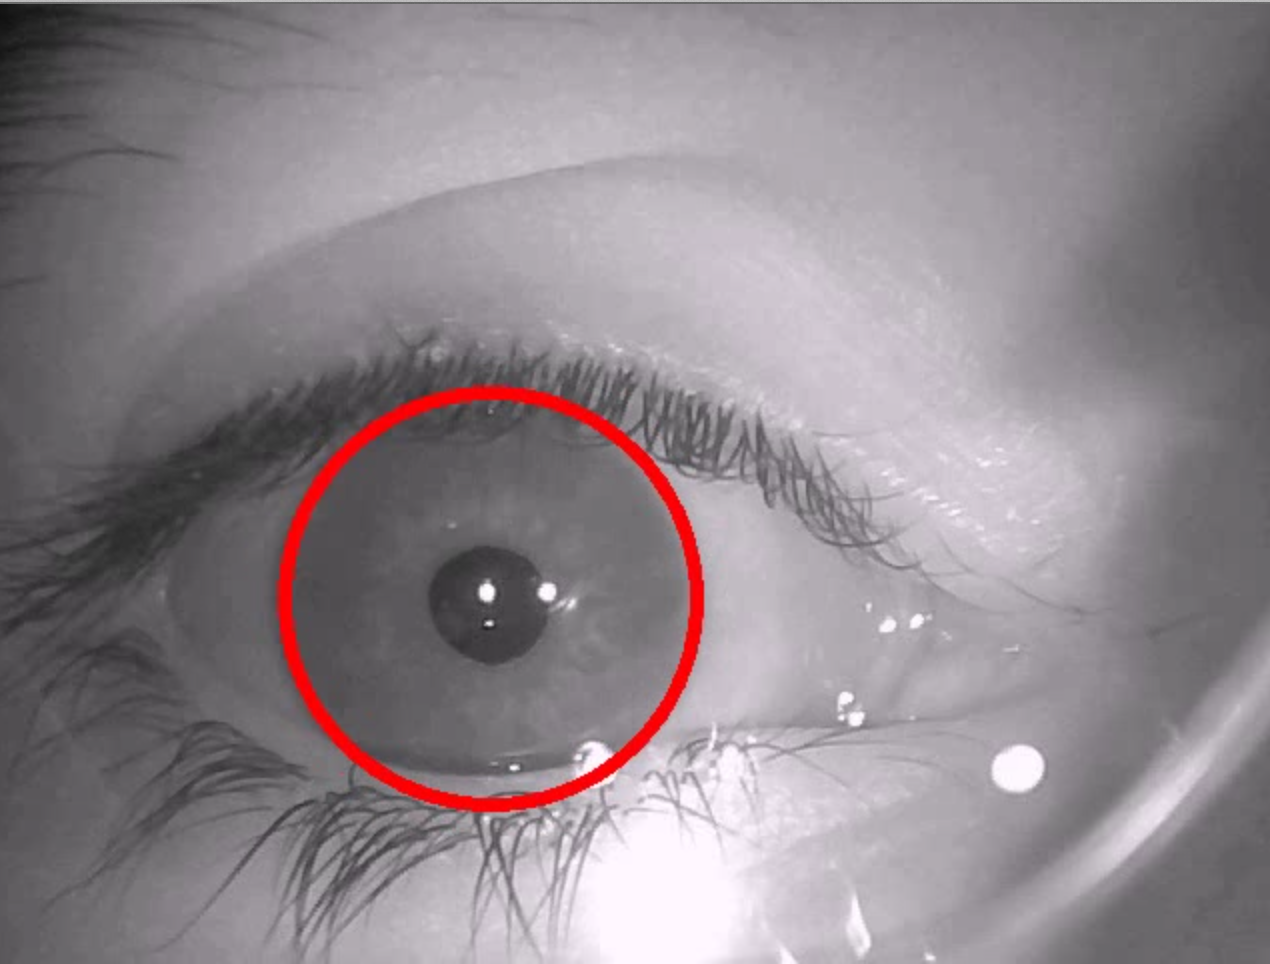
\includegraphics{pics/hough/8.png}
\caption{On this image we se why the hough transformation is really
reliable. The circle is detected even though the eyelids top and bottom
cover some of the iris. The points at the sides makes up for that and
casts enough votes on there being a full circle where the iris is,
therefore overcomming the problem that some of the iris is not visible.
\label{hough8}}
\end{figure}

\begin{figure}[htbp]
\centering
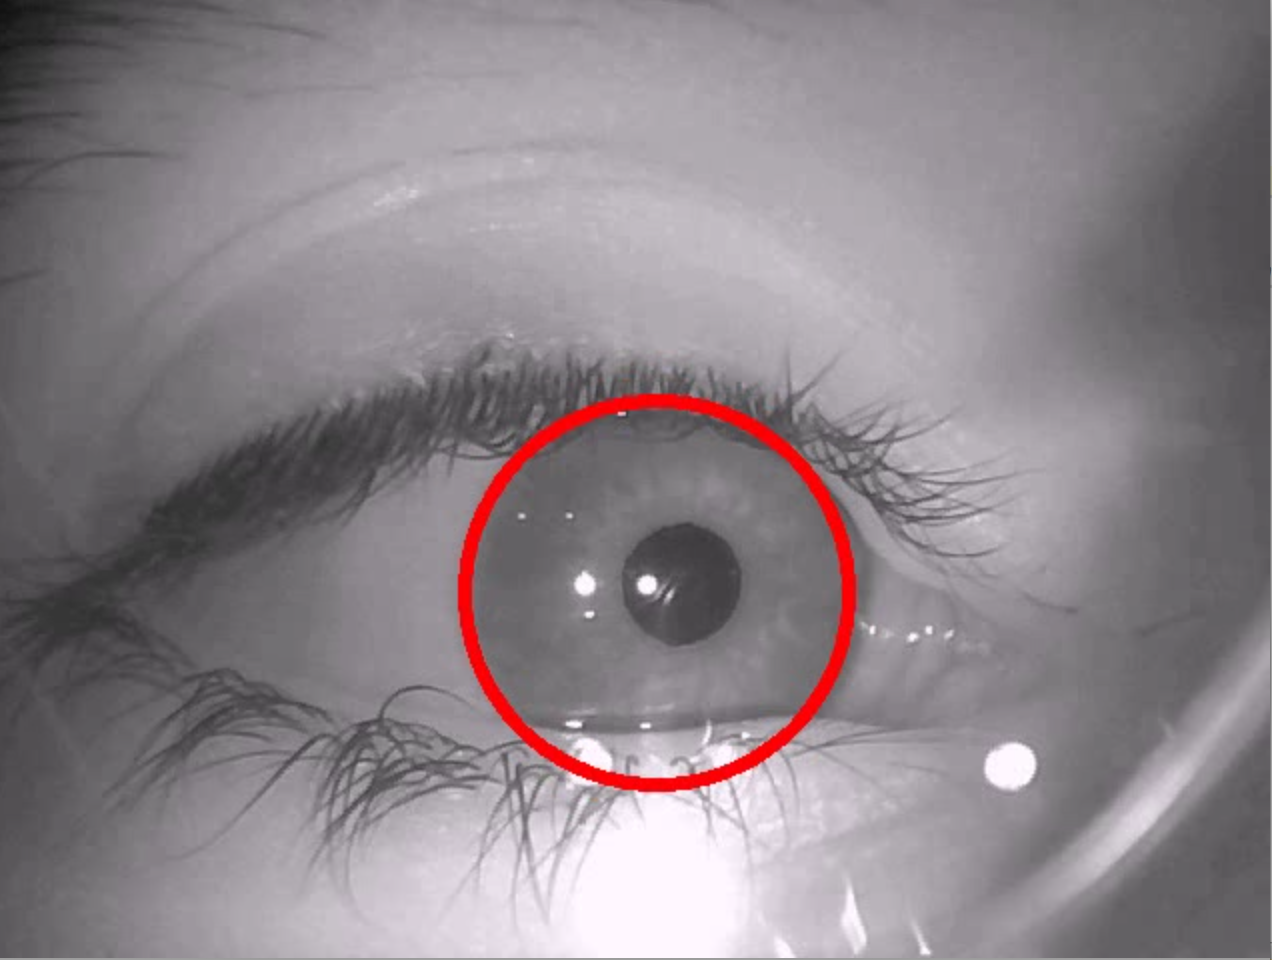
\includegraphics{pics/hough/9.png}
\caption{Even at the sides the method detects a circle, through movement
and other distractions. The circle jumps a lot, as more that one circle
is detected around the iris and they each take turns getting the most
votes, but overall a good result in these ideal circumstances.
\label{hough9}}
\end{figure}

\subsubsection{Test 2. Young Master Roed recorded 12/03/13 Pupil
Detection.}

Test settings: GaussianBlur(gray, (11,11), 11) Threshold : 50 Min/Max
size circle: 10-17

\begin{figure}[htbp]
\centering
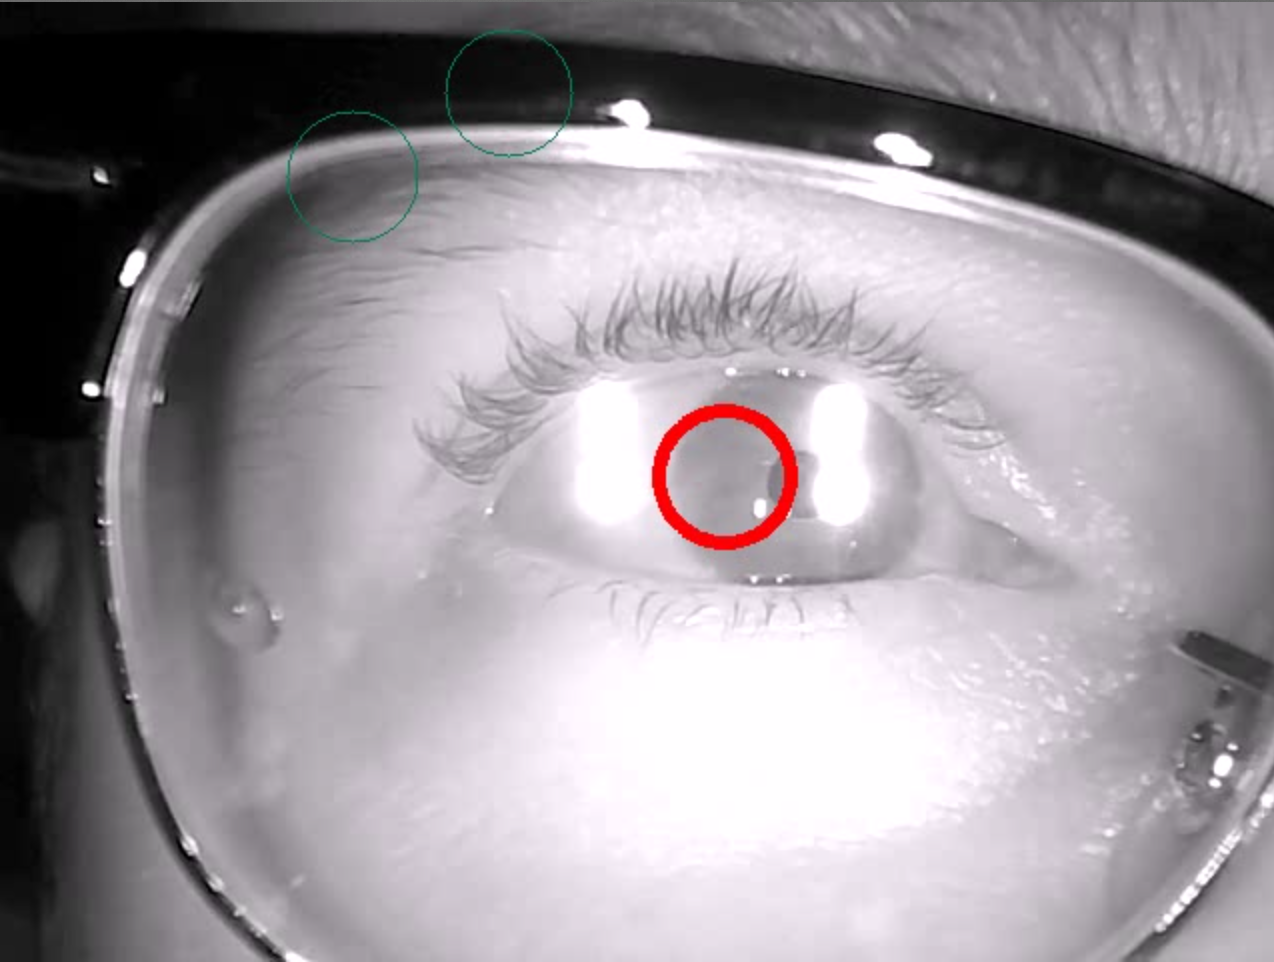
\includegraphics{pics/hough/10.png}
\caption{This image contains many distractions. The infrared lights made
a massive four reflections in the glasses covering the pupil. Instead of
finding the pupil, a part of the iris is detected as a circle edge.
\label{hough10}}
\end{figure}

\begin{figure}[htbp]
\centering
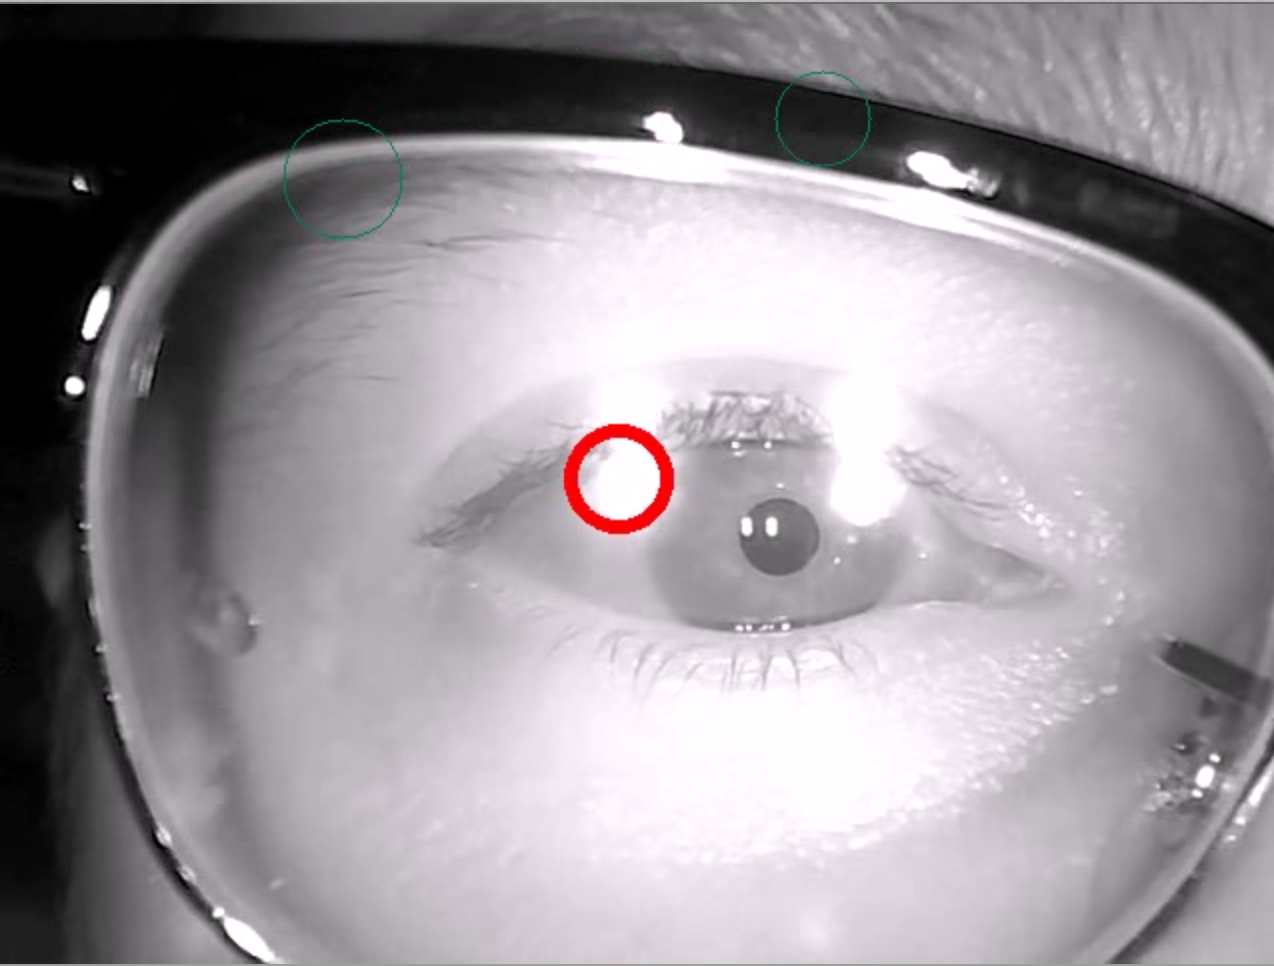
\includegraphics{pics/hough/11.png}
\caption{The distractions keep having an influence on the result, as on
this image, where the best circle match is the circular reflection of
the infrared light. THis could be compensated for by lowering the
threshold ond filtering the bads results afterwards. \label{hough11}}
\end{figure}

\begin{figure}[htbp]
\centering
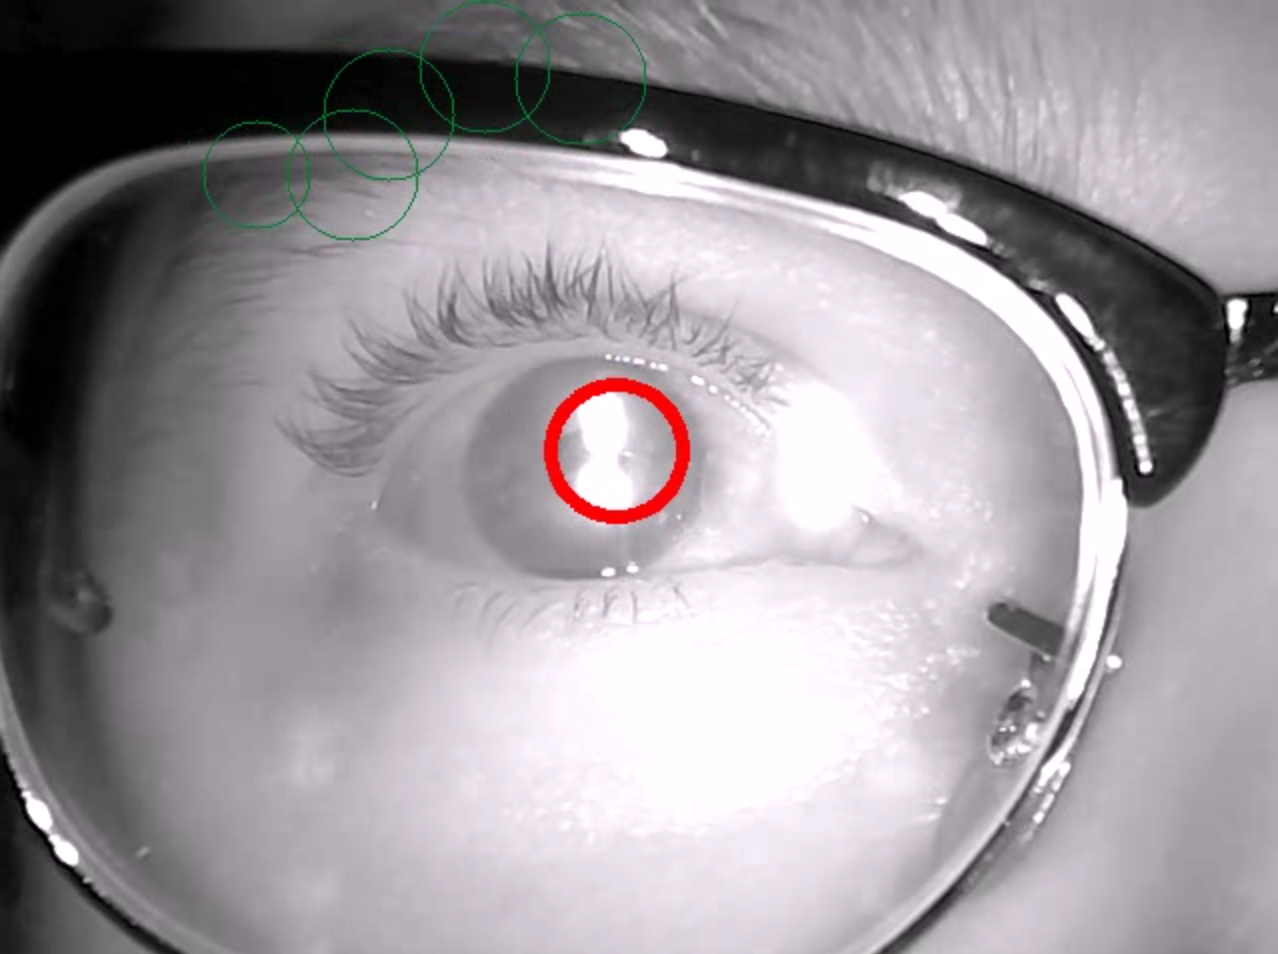
\includegraphics{pics/hough/12.png}
\caption{The distractions just proved to be too large an obstacle, as
the eye movements keeps concealing most of the pupil. Even though the
Hough method is pretty stable, it still requires a bit more controlled
environment. \label{hough12}}
\end{figure}

\subsubsection{Test 3. Young Master Roed recorded 12/03/13 Iris
Detection.}

Test settings: GaussianBlur(gray, (21,21), 11) Threshold : 120 Min/Max
size circle: 30-37

\begin{figure}[htbp]
\centering
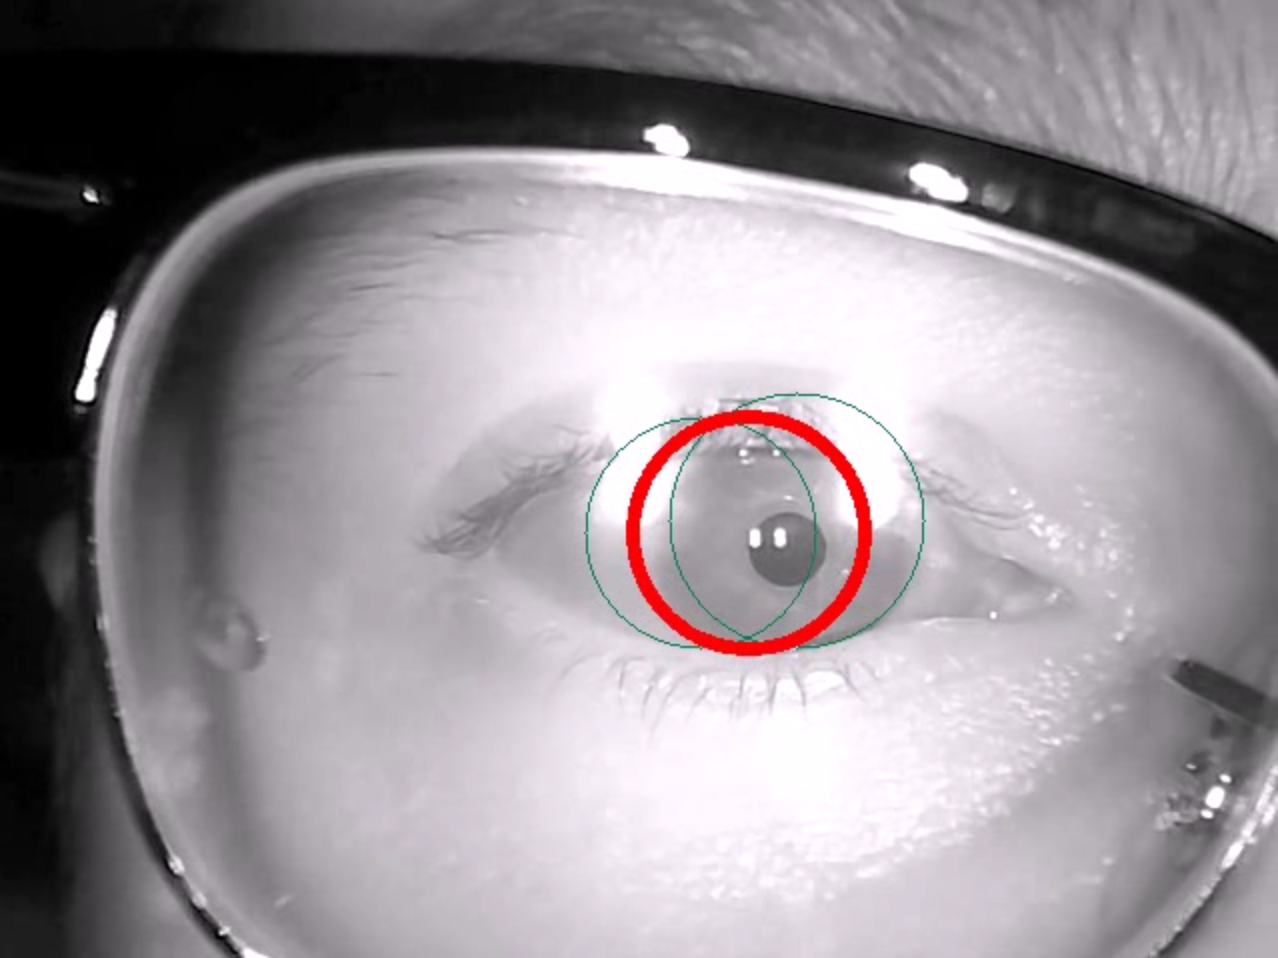
\includegraphics{pics/hough/13.png}
\caption{Finding the pupil proved a bit easier. This i probably because
the iris size is much bigger than the distraction reflection circles.
\label{hough13}}
\end{figure}

\begin{figure}[htbp]
\centering
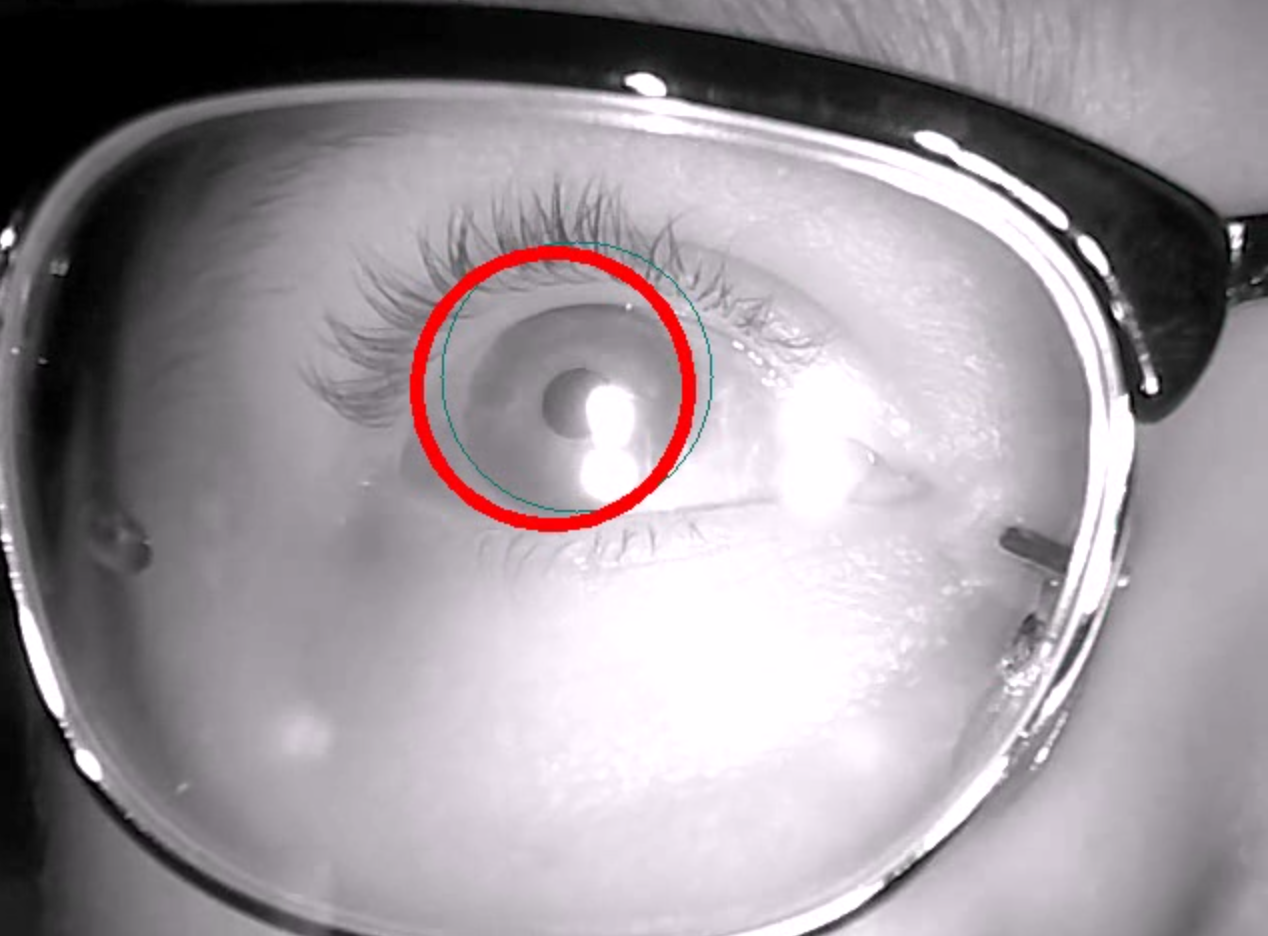
\includegraphics{pics/hough/14.png}
\caption{Looking to the sides will make the circle jump around a lot, as
it can be seen at the video. A lot of the votes still end up pat the
correct spot though. \label{hough14}}
\end{figure}

\begin{figure}[htbp]
\centering
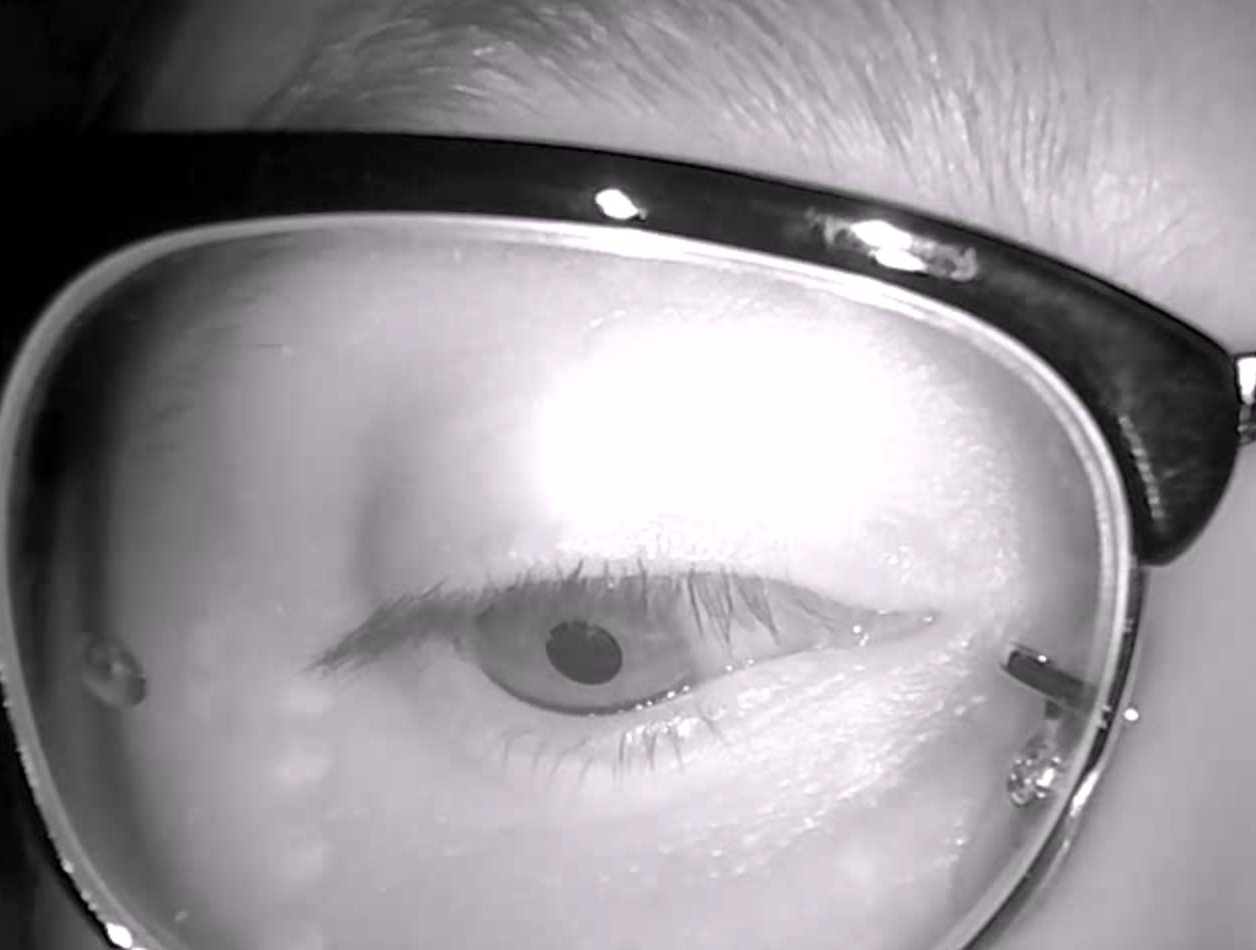
\includegraphics{pics/hough/15.png}
\caption{In this fram, there's just not enought circle edge points
visable to determine the presence of a circle. The right side of the
iris could help, but its just not enought without lowering the threshold
even further. \label{label15}}
\end{figure}

\begin{figure}[htbp]
\centering
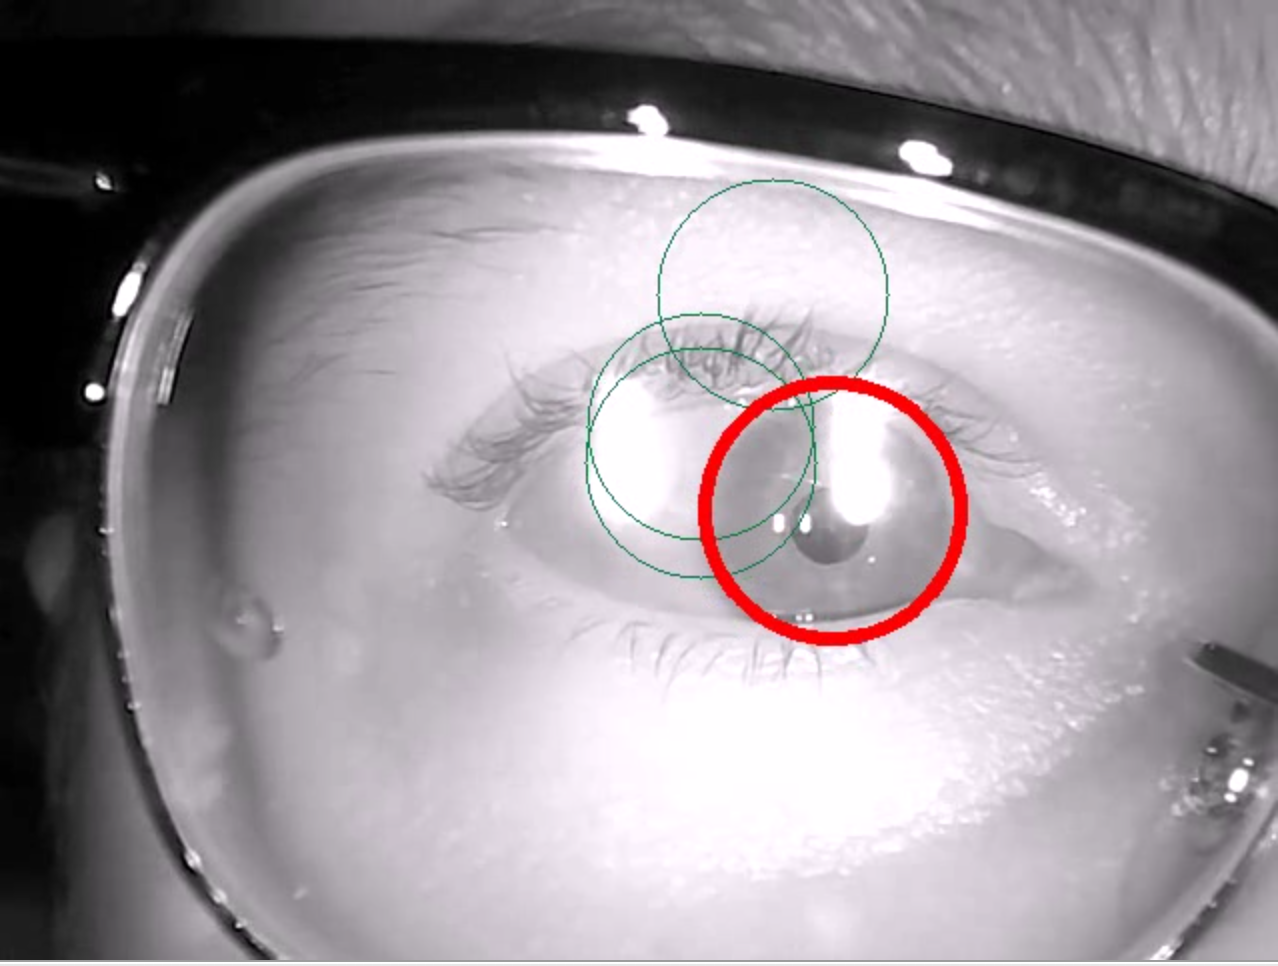
\includegraphics{pics/hough/16.png}
\caption{The threshold has been lowered even further here to 90 and
other circles appear. The most votes are still placed on the correct
circle though. \label{label16}}
\end{figure}

\subsection{Our Impressions of the technique:}

\subsubsection{When does it work?}

In an environment, where you can control the distance, resolution and
lighting of the video/image sequence, the Hough transform is very solid.
The method shines when trying to detect circles that are not complete.
As long as enough points are visible so that the circle-votes pass the
defined threshold, the method will draw the circle. This puts the method
ahead of the competition. When compared to other methods like the
thresholding method, that depends on the circularity of the found blob,
and when looking at solely using the norms for detection, being more
prone to error caused by other high gradients placed on the norm lines,
the Hough transform seems like the way to go for pupil and Iris
detection.

\subsubsection{When does it not work?}

It can be hard to set the correct threshold for the canny edge detection
as well as the minimum votes threshold, to get the correct amount of
circles. If you set it to strict it may look well with optimal
conditions, and then jump to drawing nothing as soon as the conditions
deteriorate. On the other hand, if you are less rigid with the
thresholding and min/max radius, it may look well in one image and then
jump to thousands of found circles in the next image, slowing down the
whole process. When detecting the iris we ran into some problems as
well, as the iris is not so well defined as the pupil. As it can be seen
in the video, the found iris-circle jumps a lot around. This is probably
caused by the lack of iris edge-pixels visible in the image for the
circle. The circle is found only with votes from the sides of the iris,
as the shape of the iris in reality resembles an ellipse, not a circle.

\subsection{Improving the method:}

If we were to improve the method, we would combine it with more of the
other techniques mentioned in this report. We would: Automatically
determining the pupil size with k-mean clustering. Sort out ``wrong''
results with positioning I relation to other features. Use the last
known position to filter out wrong results. (as the video is about 30
frames per second we can estimate the max movement per frame, and filter
out results that lie outside this range.)

\subsection{Conclusion:}

Out of the box, Hough transform works quite well for pupil/iris
detection, its robust even if the image contains noise (salt and pepper,
not large distractions), and when considering that the method allows for
searching for multiple times appearence of a shape in a single pass its
both fast and reliable.


\end{document}
